\graphicspath{{Figures/Systematics/}}

\section{Systematics}

In the following we list and discuss the different sources of uncertainties entering into account in the \Raa computation. 
The main sources are those on the pp reference and the signal extraction.
A summary table is provided at the end of the section (\ref{tablesys}).

\subsection{\label{sysSigExtr}Signal extraction systematic}

\paragraph{}
Several tests are performed to estimate the systematic uncertainty related to the signal and background shapes as well as the fixed parameters like the \upsp width.
The different tests are presented thereafter.
 
\paragraph{Set of tails}
Since the CB2 function reproduces well the signal (>99\%), only the sets of tails fixed on MC are tested.
For that we have extracted, via the same fit procedure as in data, the tail parameters from the invariant mass of reconstructed \ups signal generated in MC simulations.
A pure \ups MC sample has been produced with Geant4 transport codes to be compared to the embedding MC sample based on Geant3 transport code.
The sets of tails extracted from the integrated spectra are shown on figure \ref{tails}
Due to the small statistics of signal in raw data and the quite high resolution of the pic the effect of the tails on the amount of measured \ups is small.
Integrated over \pt and $y$ intervals the difference is less than 1\% level, reaching a maximum of 3\% as a function of $y$.
Note that an other set of tails extracted in pp data at $\sqrtS=13$\;TeV for which the S\/B ratio and integrated luminosity is much higher has been tested.
Nevertheless the parameters being not enough constrained the results return by the fit was unrealistic.
That was the same by letting the tails free.
The centrality and rapidity dependence of the tail parameters has been study in embedding MC sample.
The results are reported on the figure \ref{evoltails}.
We observed a significant variation as a function of $y$ and a small evolution of the right tail as a function of centrality which is not significative.
Finally two sets of tails are used i(pure \ups MC with G4 and embedding MC with G3 ) in the evaluation of the signal extraction systematic.
Their rapidity dependence is taken into account and the set extracted from the integrated centrality classes (0-90\%) is used for all centrality classes.

\begin{figure}[!b]
\begin{center}
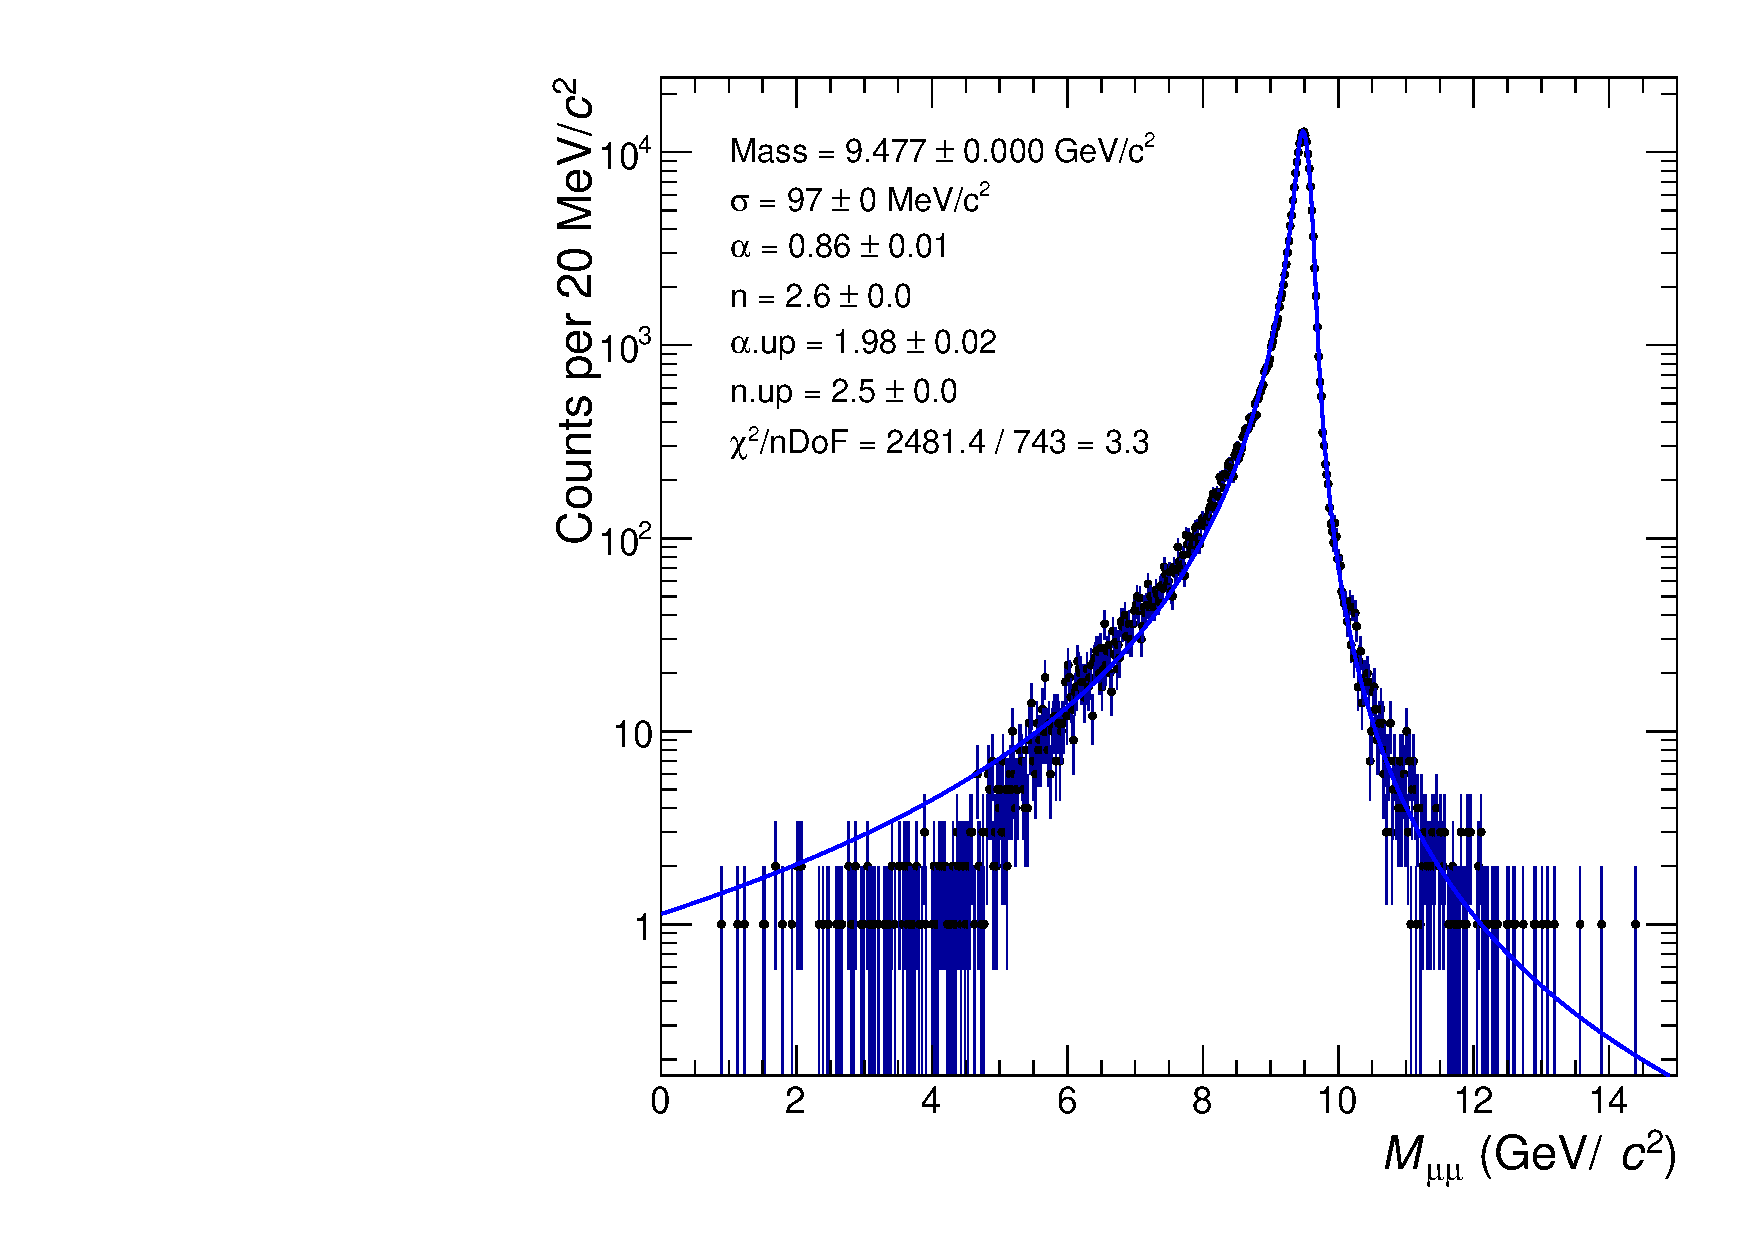
\includegraphics[width=6cm]{/Tails/Integrated_embedding.pdf}
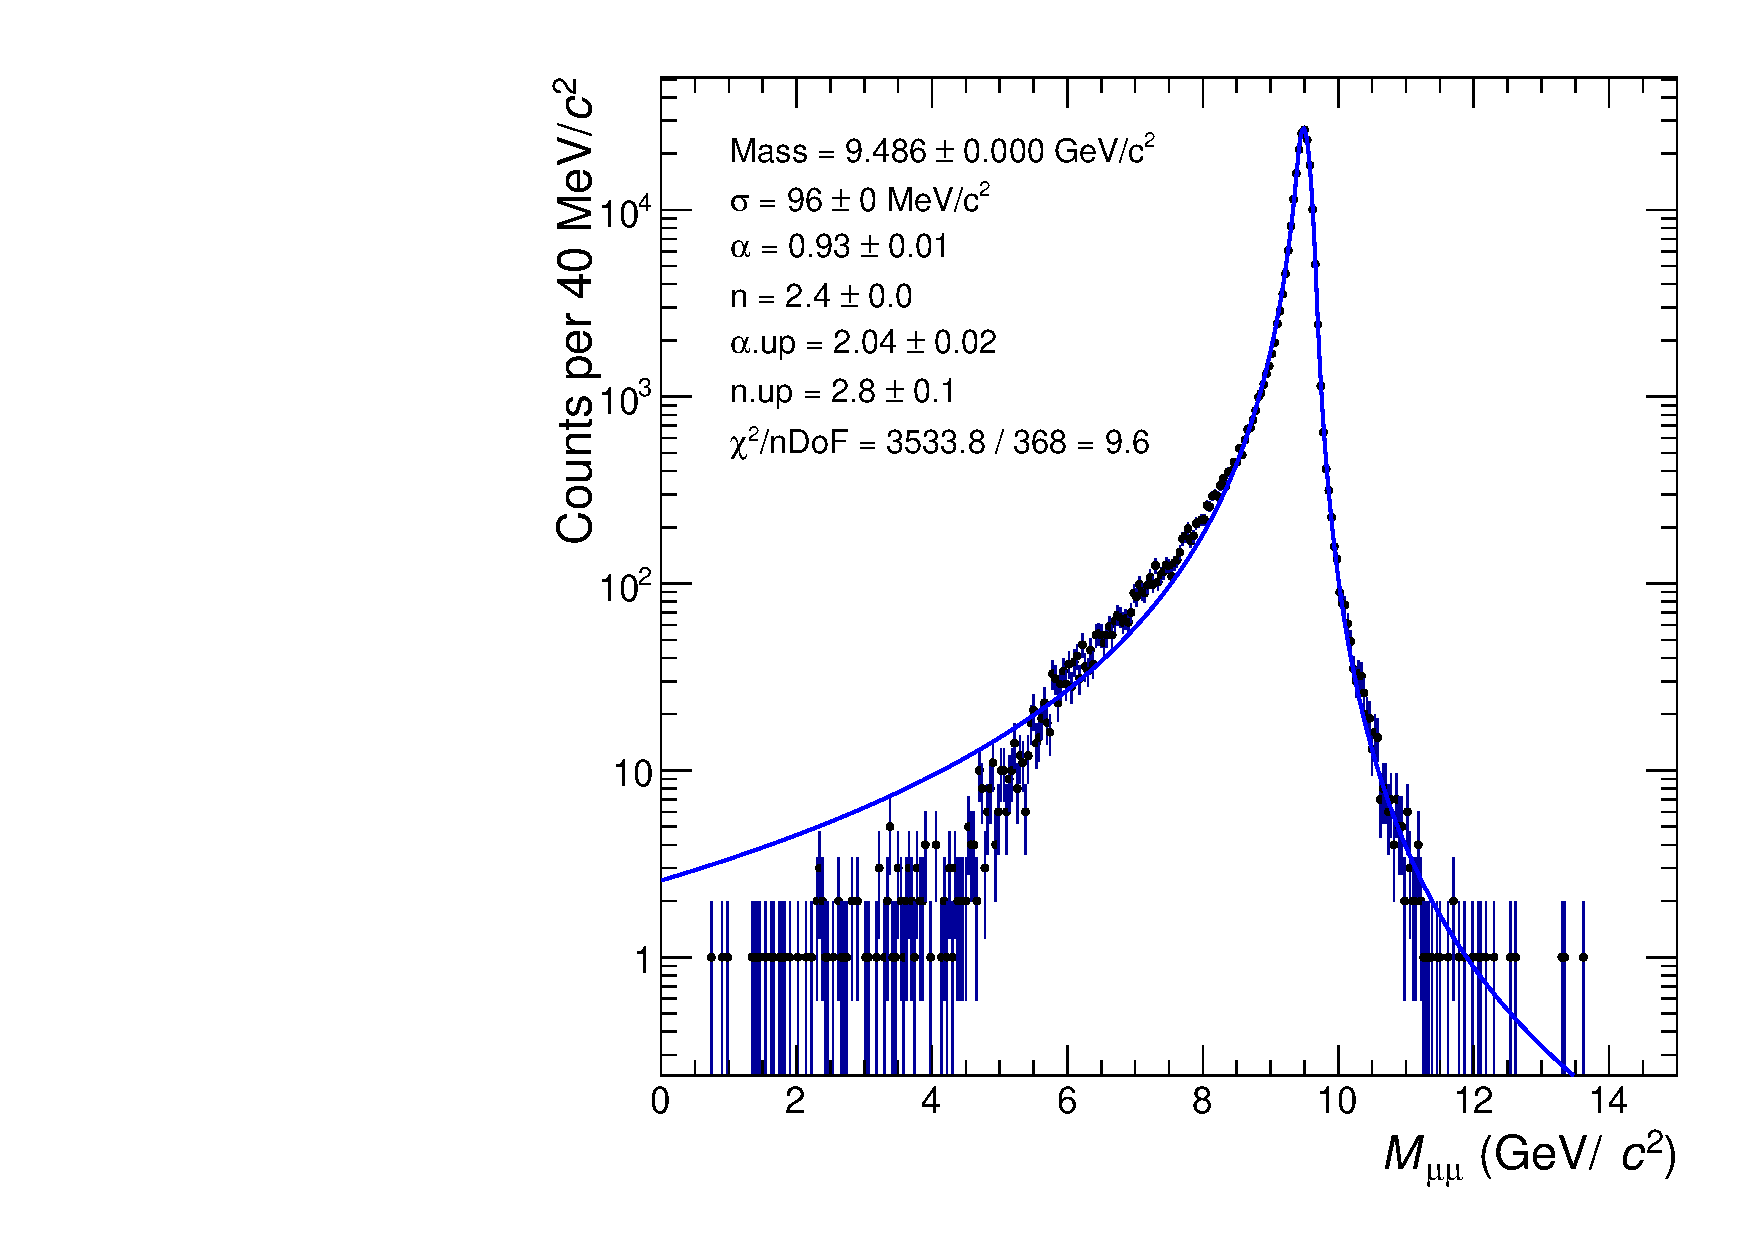
\includegraphics[width=6cm]{/Tails/integratedG4.pdf}\\
\end{center}
\caption{\label{tails}Fit of the signal shapes obtained in embedding (left) and pure (right) \ups MC samples with a CB2 function.}
\end{figure}

\begin{figure}[!t]
\begin{center}
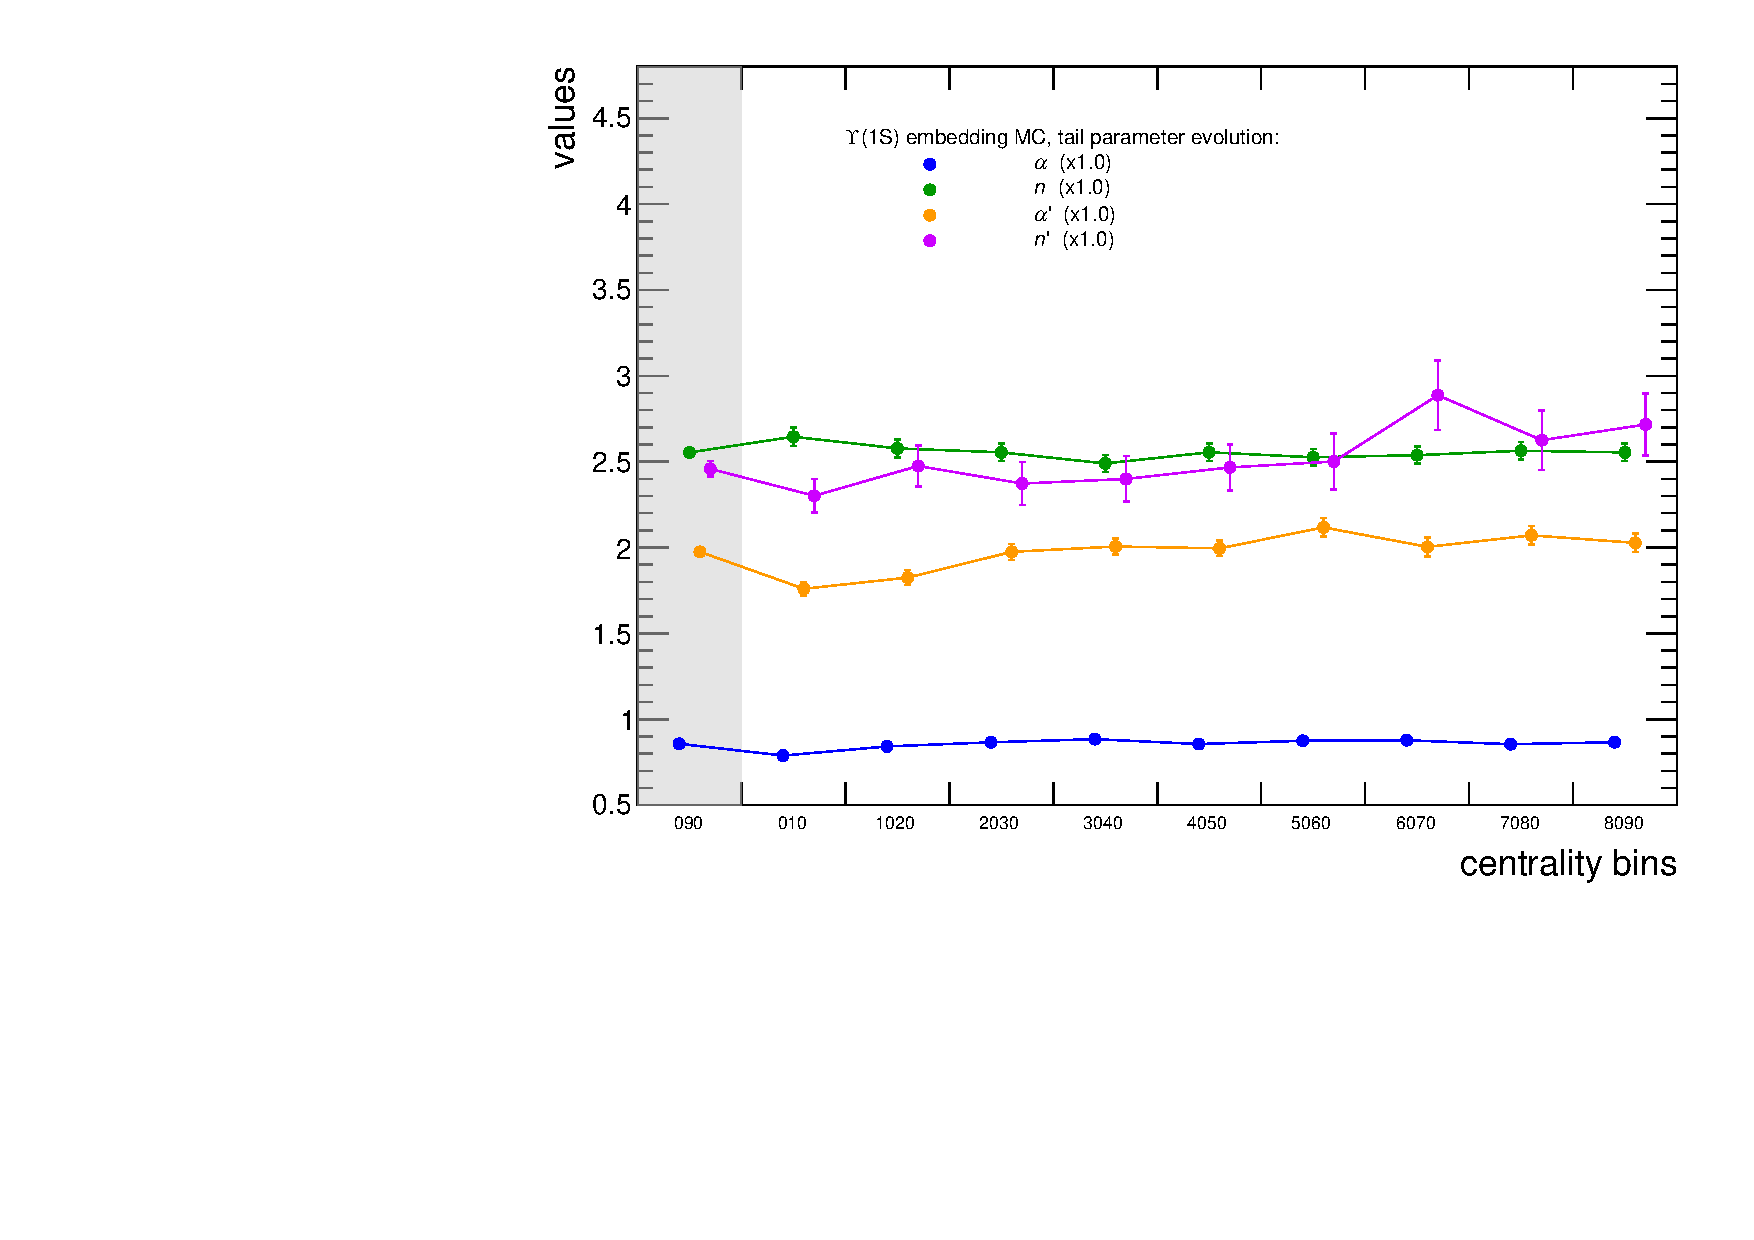
\includegraphics[width=6cm]{/Tails/Evol_ParamTails_cent_SimuUpsilon1S.pdf}
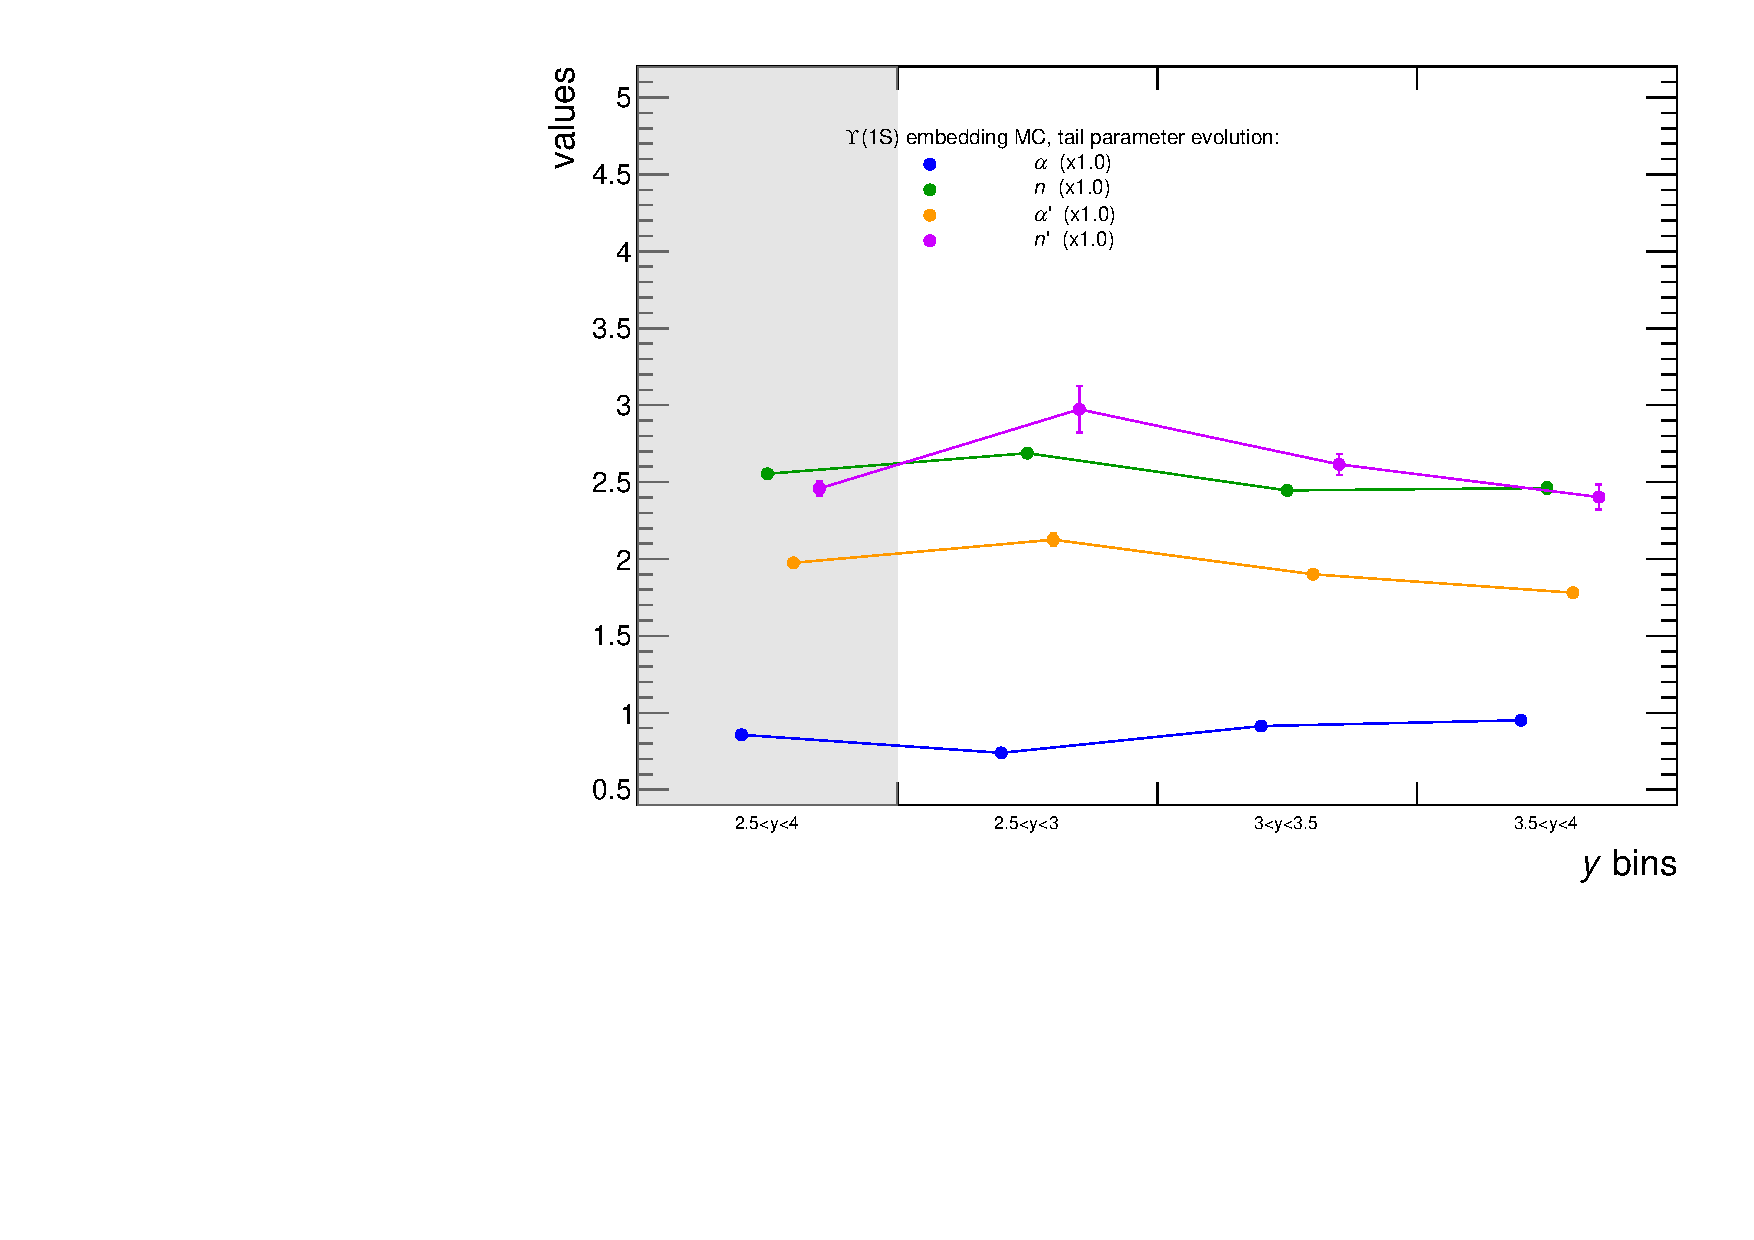
\includegraphics[width=6cm]{/Tails/Evol_ParamTails_y_SimuUpsilon1S.pdf}
\end{center}
\caption{\label{evoltails}Centrality (left) and rapidity evolution of the tail parameters. The grey bands correspond to the integrated result.}
\end{figure}

\paragraph{$\boldsymbol{\upsp \text{ and } \upspp}$ widths}
Due to the poor S/B ratio of higher resonances one have to fix their width.
As explained in section \ref{signalextraction}, the widths are scaled to the \ups width, left it free, by the ratio obtained in MC.
In both MC samples these ratio are very close and $\sigma_{\upsp}/\sigma_{\ups}=1.03$ and $\sigma_{\upspp}/\sigma_{\ups}=1.06$.
To test the validity of this scaling one vary the higher resonance widths by the relative uncertainty of the \ups width parameter return by the fit in data.
Note that it has been testing to let the \upsp and \upspp width free in data, unfortunately the signal is too small to constrain significantly the width parameter giving an uncertainty beyond 100\%.
A maximum uncertainty of 10\% is observed for the \ups and used to perform two tests in $\pm1\sigma$ of the scaled \upsp and \upspp widths in the same direction for both.
Since the \upsp and \upspp signals do not affect the \ups one as a fonction of centrality and rapidity these two tests are performed only for the integrated invariant mass spectrum.

\paragraph{Background function} 
To test the background reproduction several ad hoc functions are used.
As in previous \upsi analyses, a sum of two exponential and a sum of two power law are used.
Both functions return a good $\chi^2$ never exceeding 1.8.
The observed variation goes up to 10\% for the integrated spectrum.    

\paragraph{Fitting range} 
To check the stability of the fitting procedure an additional test by varying the fitting range of the dimuon invariant mass spectrum is 
Thus different ranges have been tried (narrow, wide, etc).
The results reported in this note are obtained by operating two fitting ranges: $6<m_{\mu\mu}<13$ GeV/$c$ and $7<m_{\mu\mu}<14$ GeV/$c$.
The observed variation goes up to 7\% for the integrated spectrum.   

\paragraph{\label{mixing}Event mixing}
Finally, in order to improve the reproduction of the background shape the event mixing technic has been performed.
From our past experience, it has been demonstrated that the single muon low \pt threshold (CMSL7) dataset is the best one to reproduce the like sign muon pairs invariant mass distribution obtained by analyzing the CMUL7 or CMLL7 triggered events.
9 pools of events are formed according to their centrality (interval of 10\%) in order to mix similar events in term of multiplicity for instance.
That procedure is a run by run basis to account for the time evolution of the apparatus.
It has been checked that the merging of the mixed spectra over the run numbers has a negligible effect whether it is made before or after normalization.
It is therefore realized before. 
Furthermore, it has also been checked that the best normalization method is the one based on the like sign muon pairs distributions such as, unlike the integral method of the :
\begin{align*}
\int_{5}^{14}{ N^{+-}_{mix}\, dM}&=\int_{5}^{14}{ 2R\sqrt{N^{++}_{raw}N^{--}_{raw}}\, dM} \\
\text{with} \,\;\  R&=\frac{ N^{+-}_{mix} }{ 2\sqrt{N^{++}_{mix}N^{--}_{mix}} },
\end{align*} 
which accounts for the difference acceptances between $\mu^+$ and $\mu^-$.
Due to the high momentum carried out by the muon entering in the high mass region off the invariant mass, the $R$ factor is flat and equal to 1 as a function of the dimuon invariant mass.
Thus the determination of the normalization factor can be achieved on the full mass range of the fit including the upsilon mass region.
Note that due to the decreasing trend of the CMSL7 event distribution as a function of centrality, the normalisation procedure should be apply per centrality pool before any merging of centrality classes. 
The resulting normalized mixed spectra are compared on figure \ref{normalization} to the the raw ones as a function of the invariance mass (first raw), the dimuon \pt (second raw) and $y$ (third raw) for positive like sign dimuon (first column), negative like sign dimuon (second column) and the opposite sign dimuon (third column).
We can appreciate the good reproduction of the background  by looking the flat ratios obtained between like sign dimuon distributions.
Finally the normalized mixed spectrum is subtracted to the raw one.
The resulting  subtracted invariant mass distributions are then used as alternative input distributions for estimating the signal extraction systematic uncertainty.
All the tests described above are applied for which only the ad hoc background functions change to either one exponential or one power law.

\begin{figure}[!t]
\begin{center}
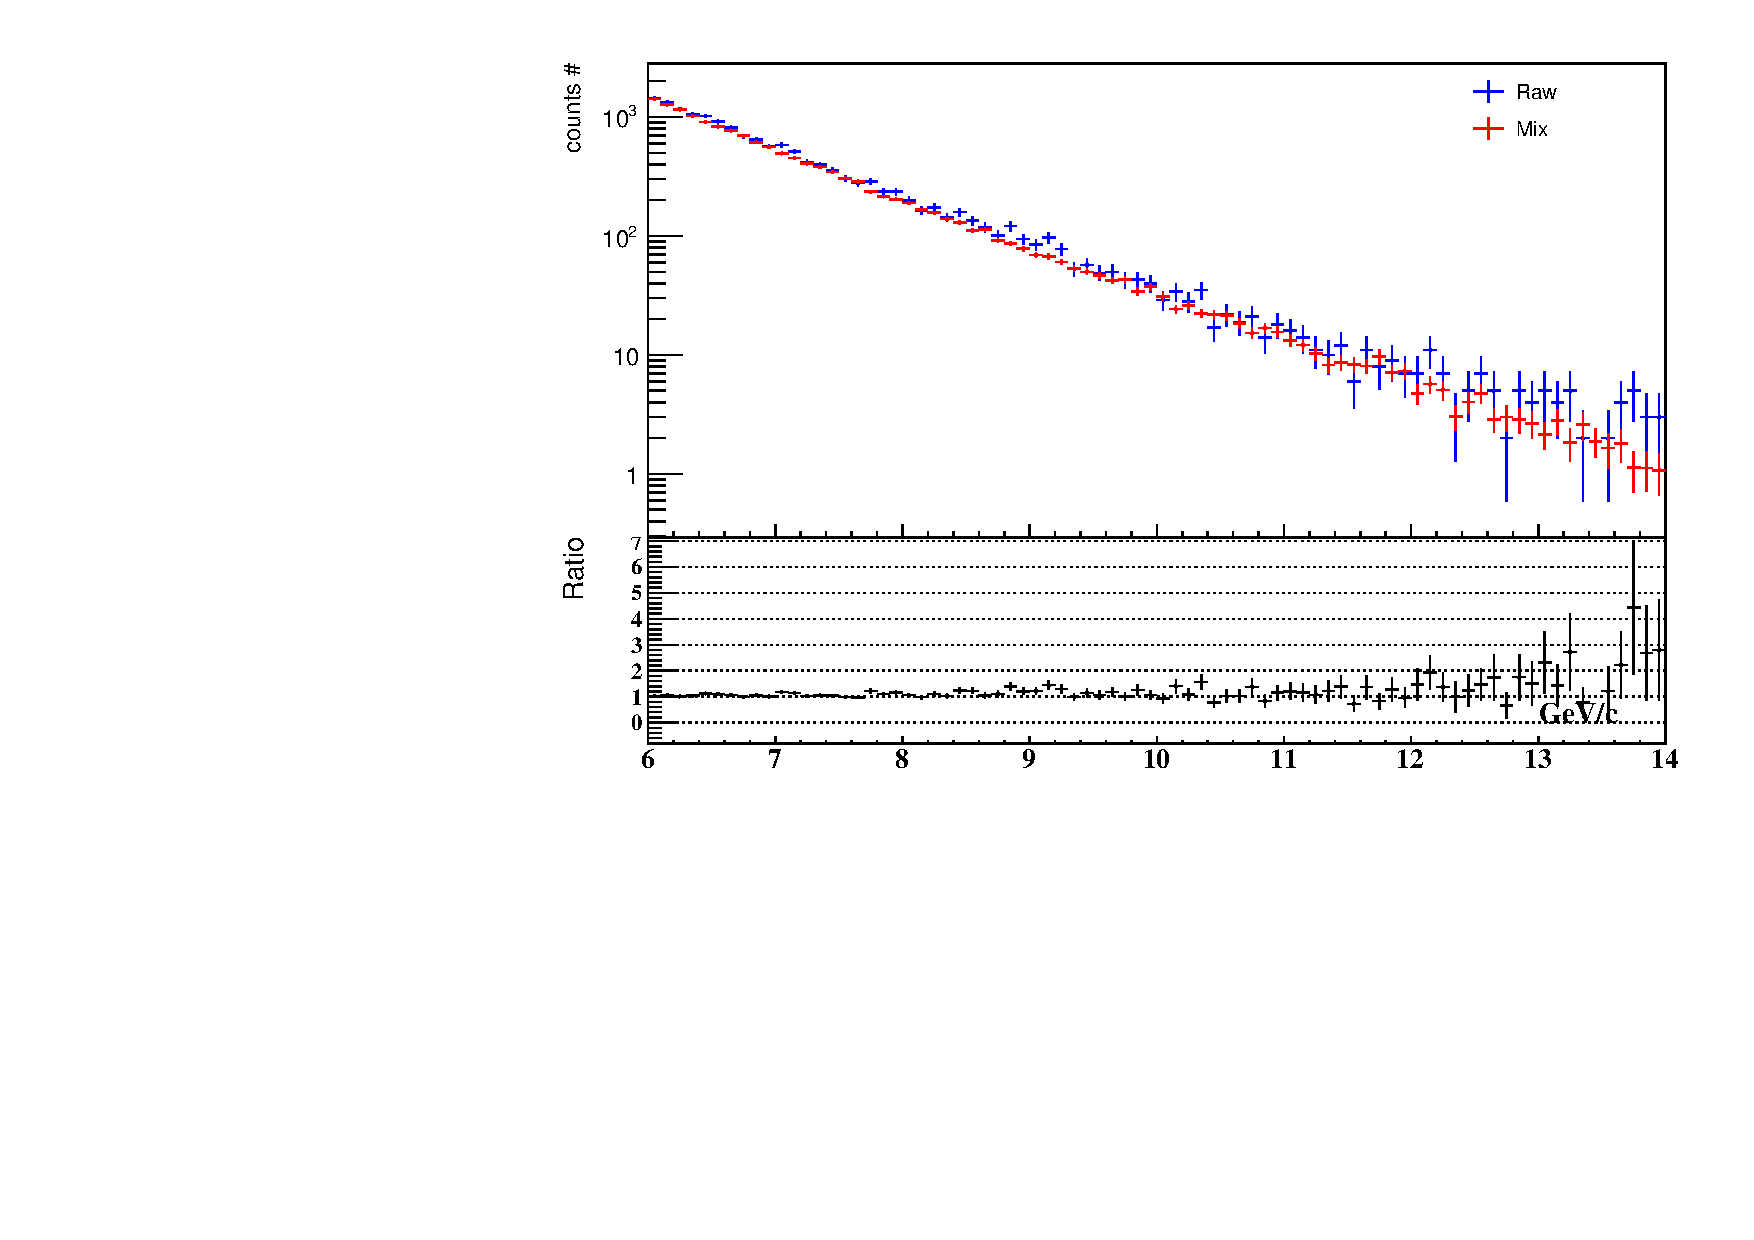
\includegraphics[width=5cm]{/Mixing/M_PP.pdf}
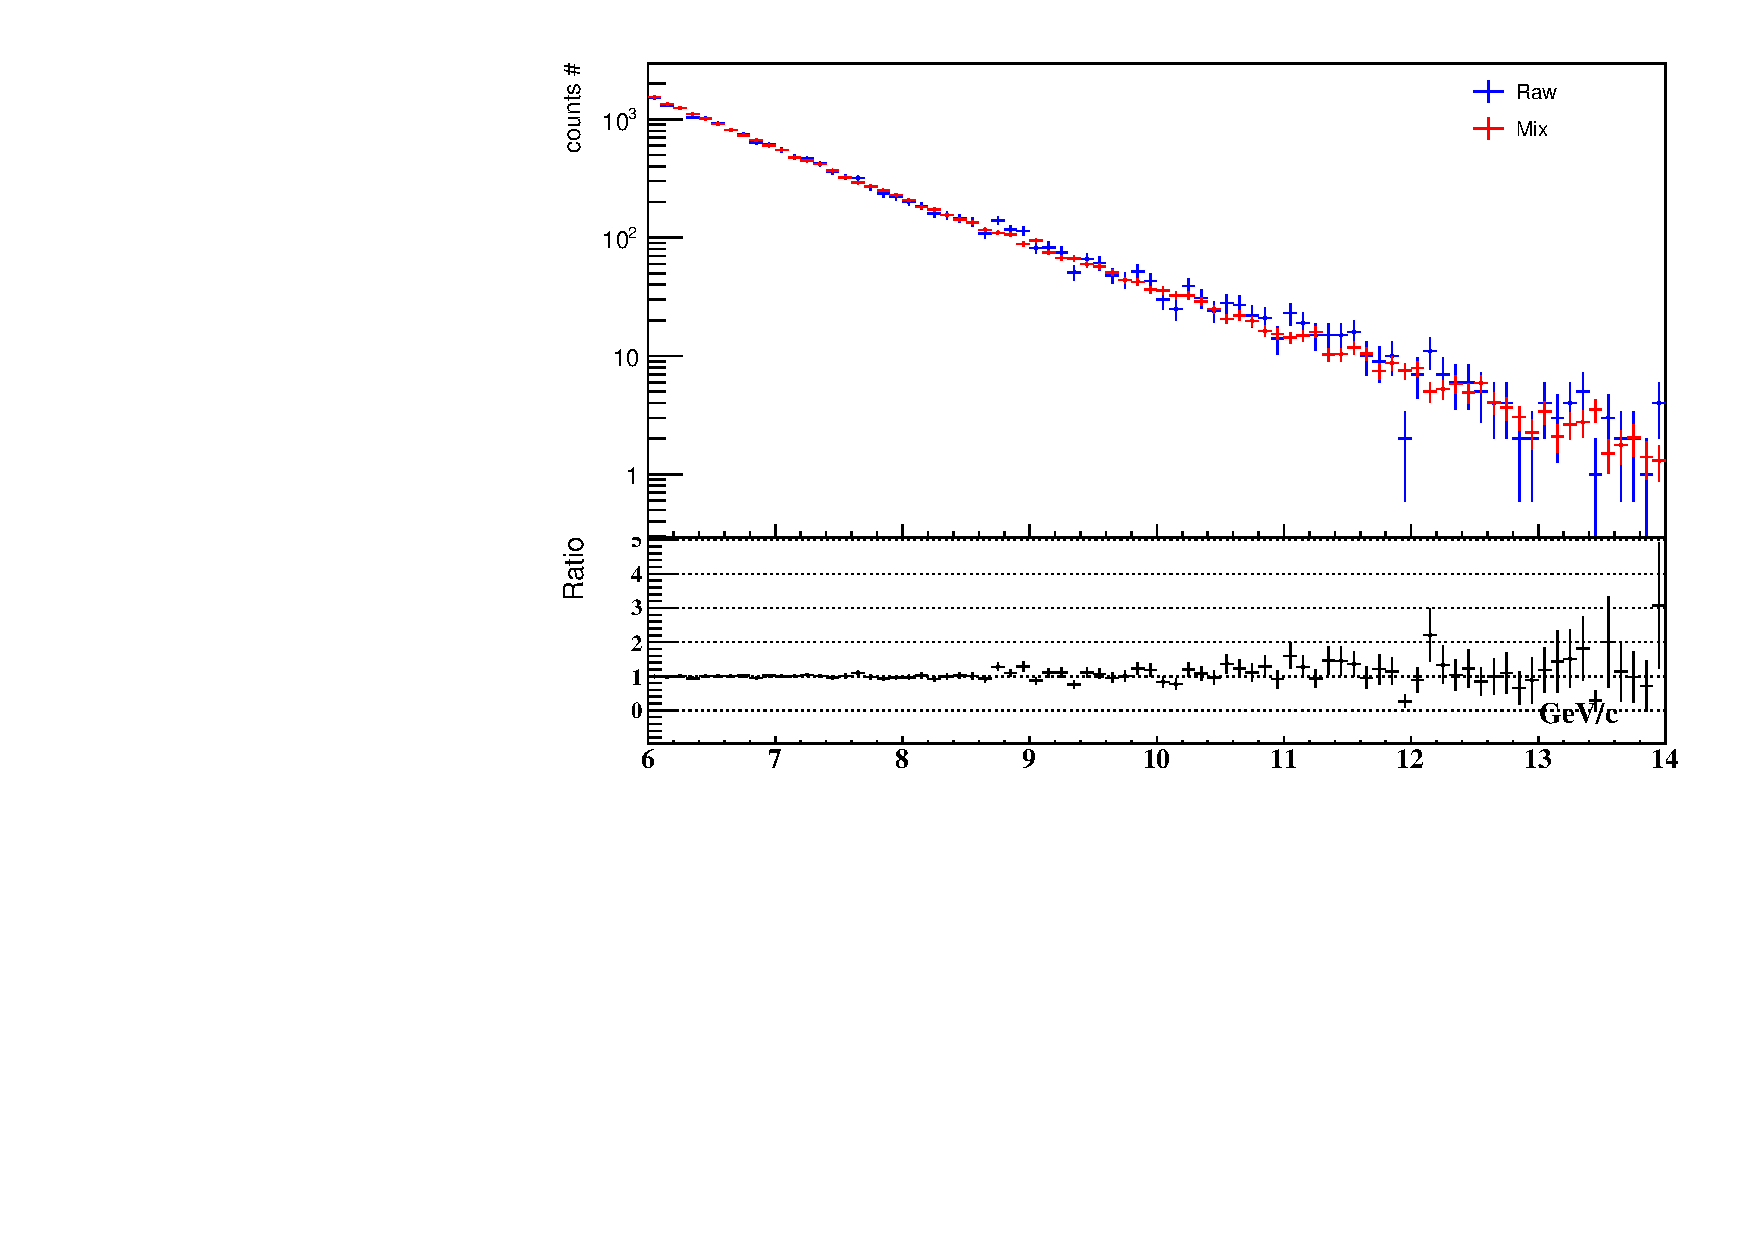
\includegraphics[width=5cm]{/Mixing/M_MM.pdf}
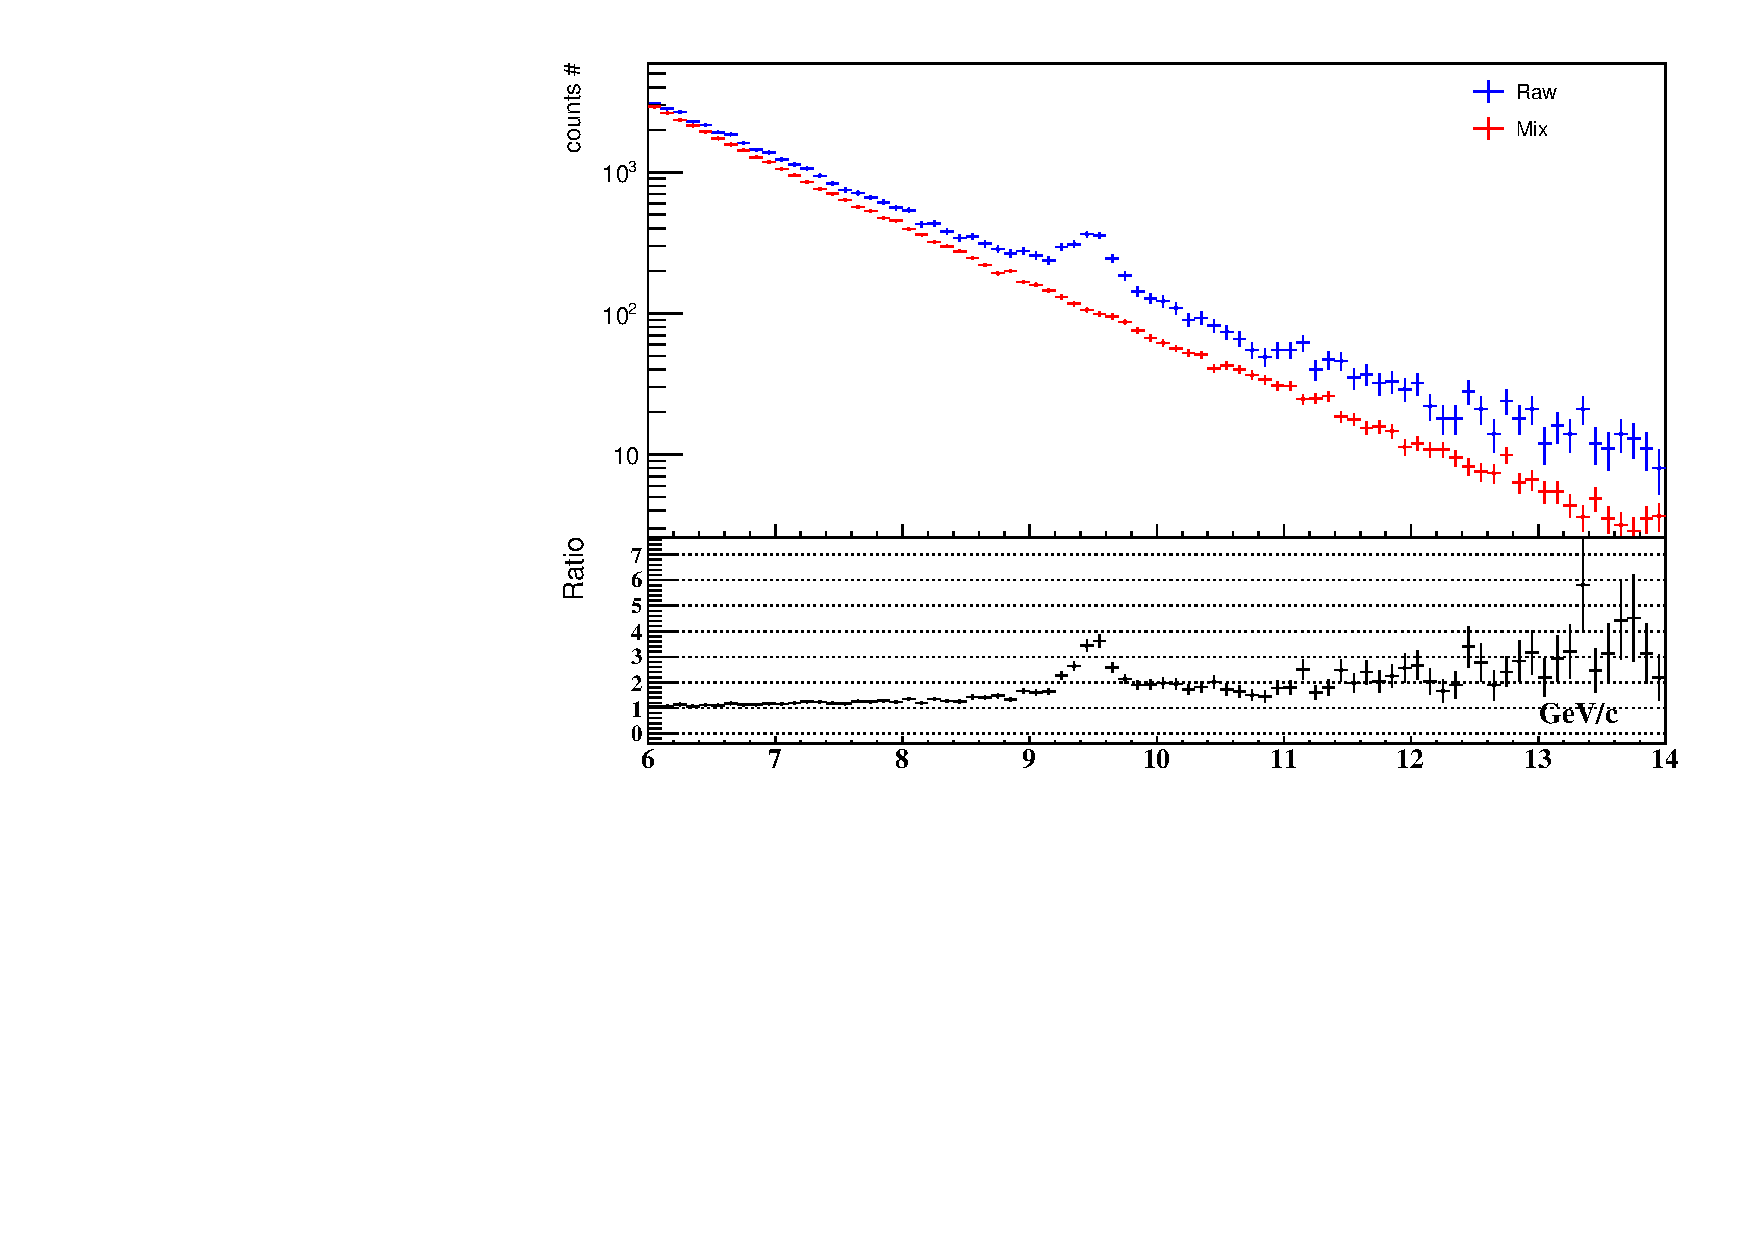
\includegraphics[width=5cm]{/Mixing/M_PM.pdf}\\
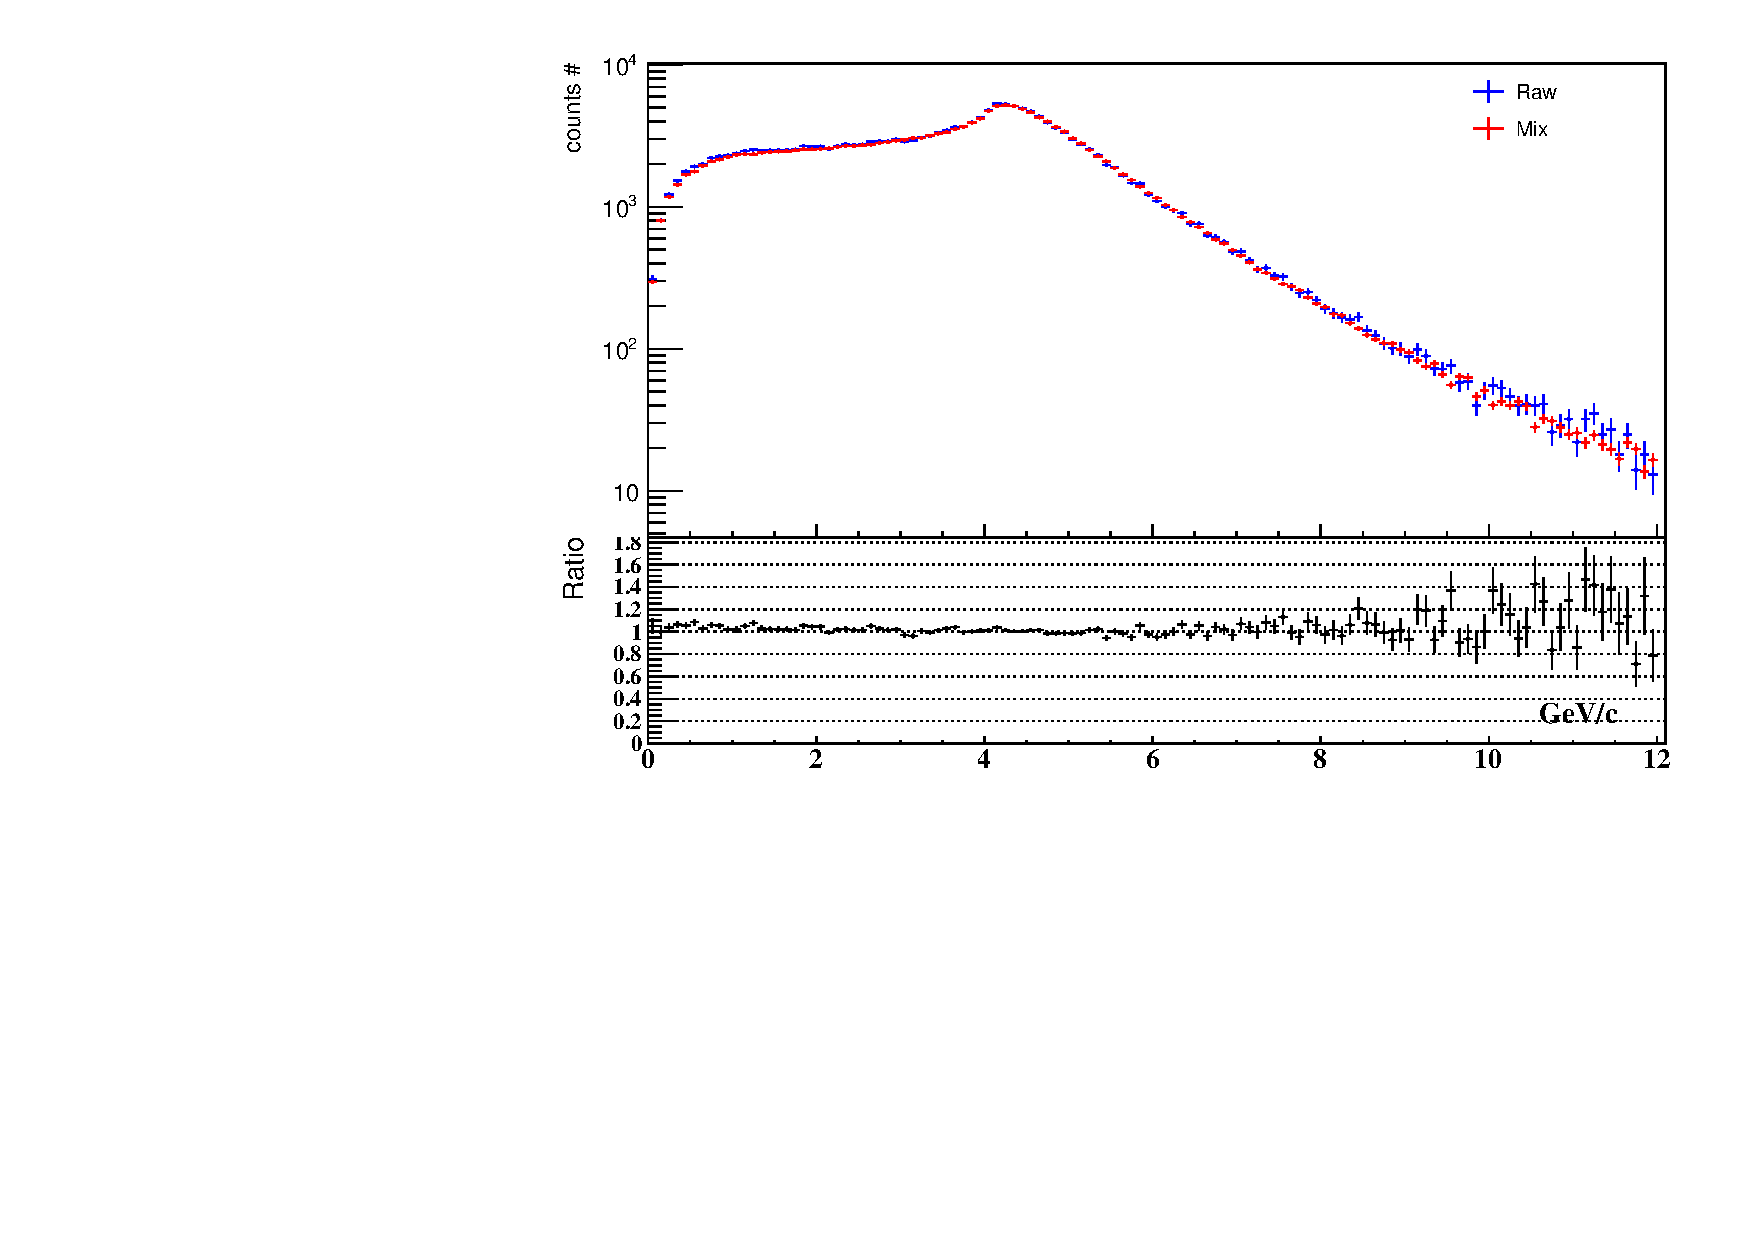
\includegraphics[width=5cm]{/Mixing/Pt_PP.pdf}
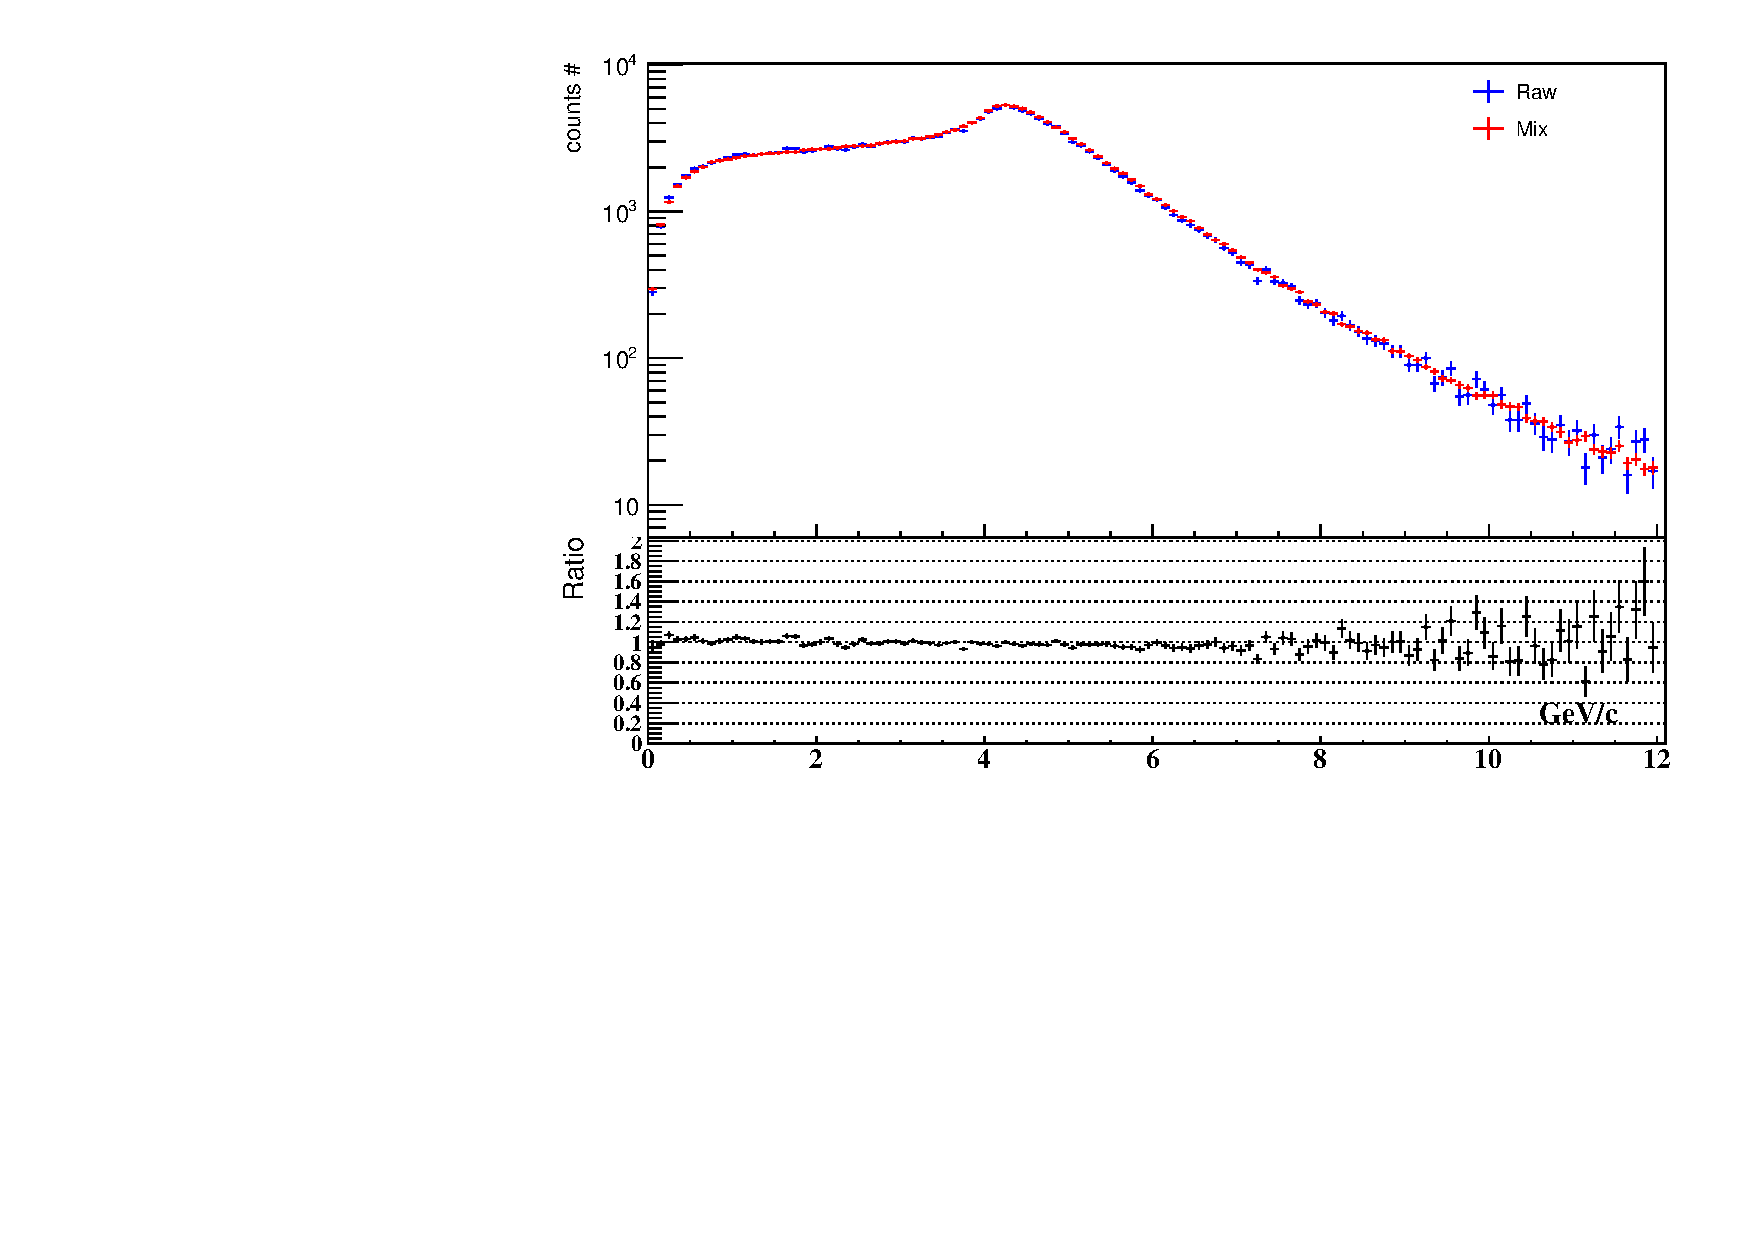
\includegraphics[width=5cm]{/Mixing/Pt_MM.pdf}
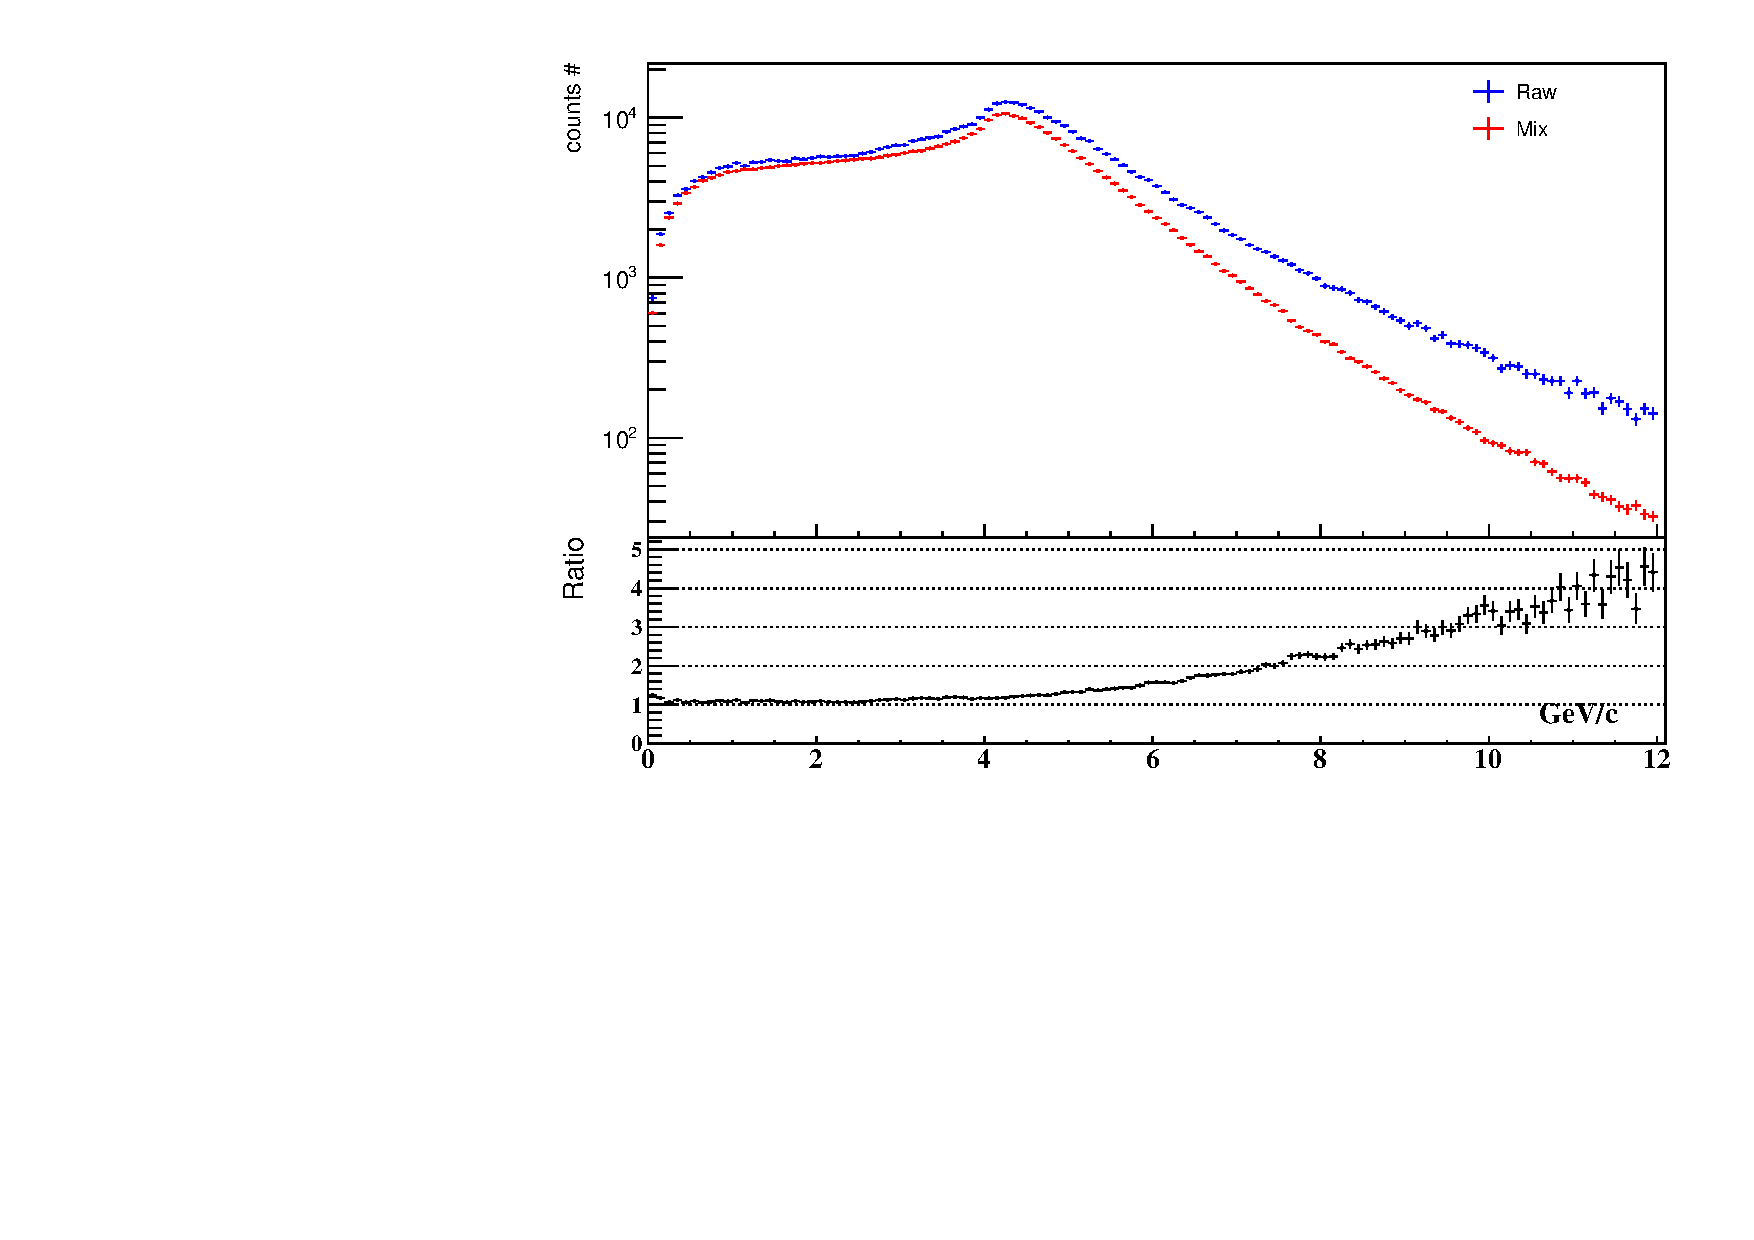
\includegraphics[width=5cm]{/Mixing/Pt_PM.pdf}\\
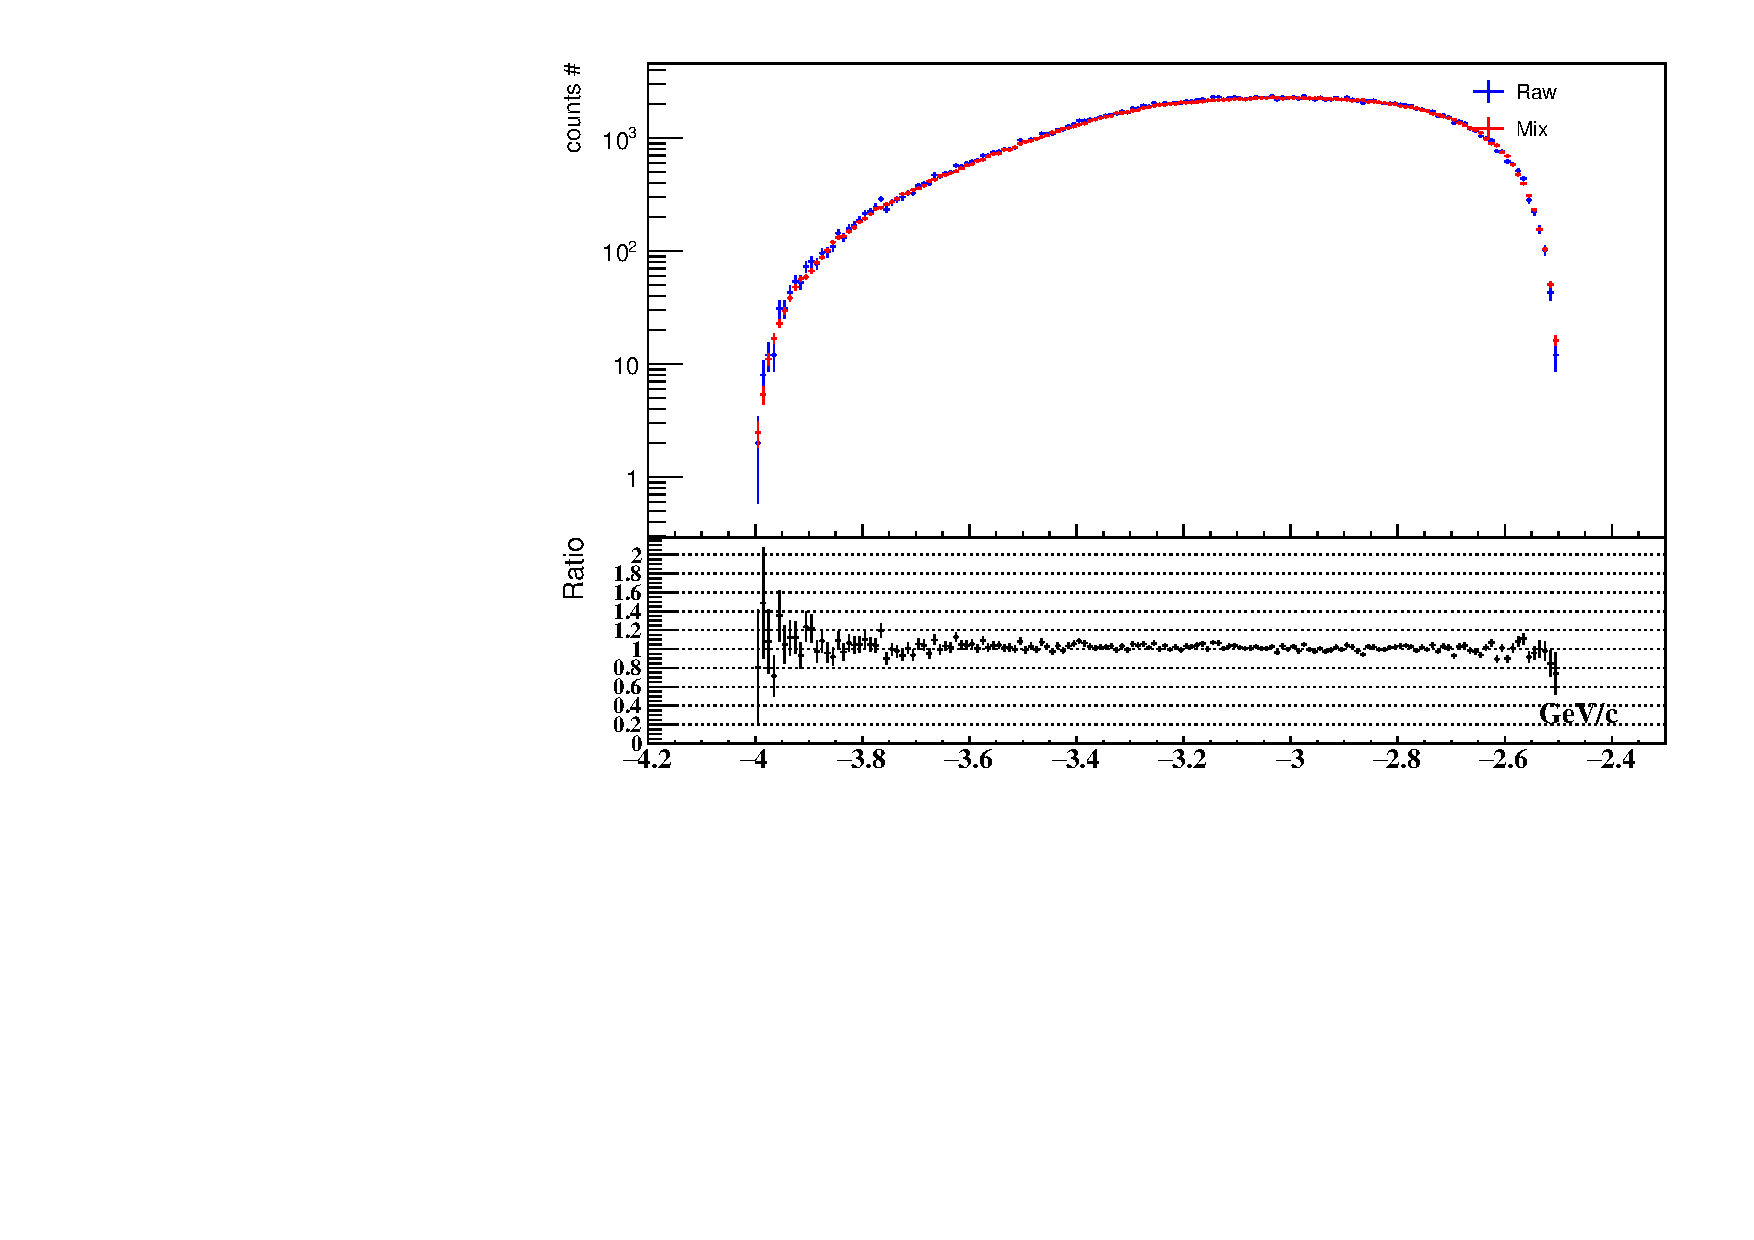
\includegraphics[width=5cm]{/Mixing/Y_PP.pdf}
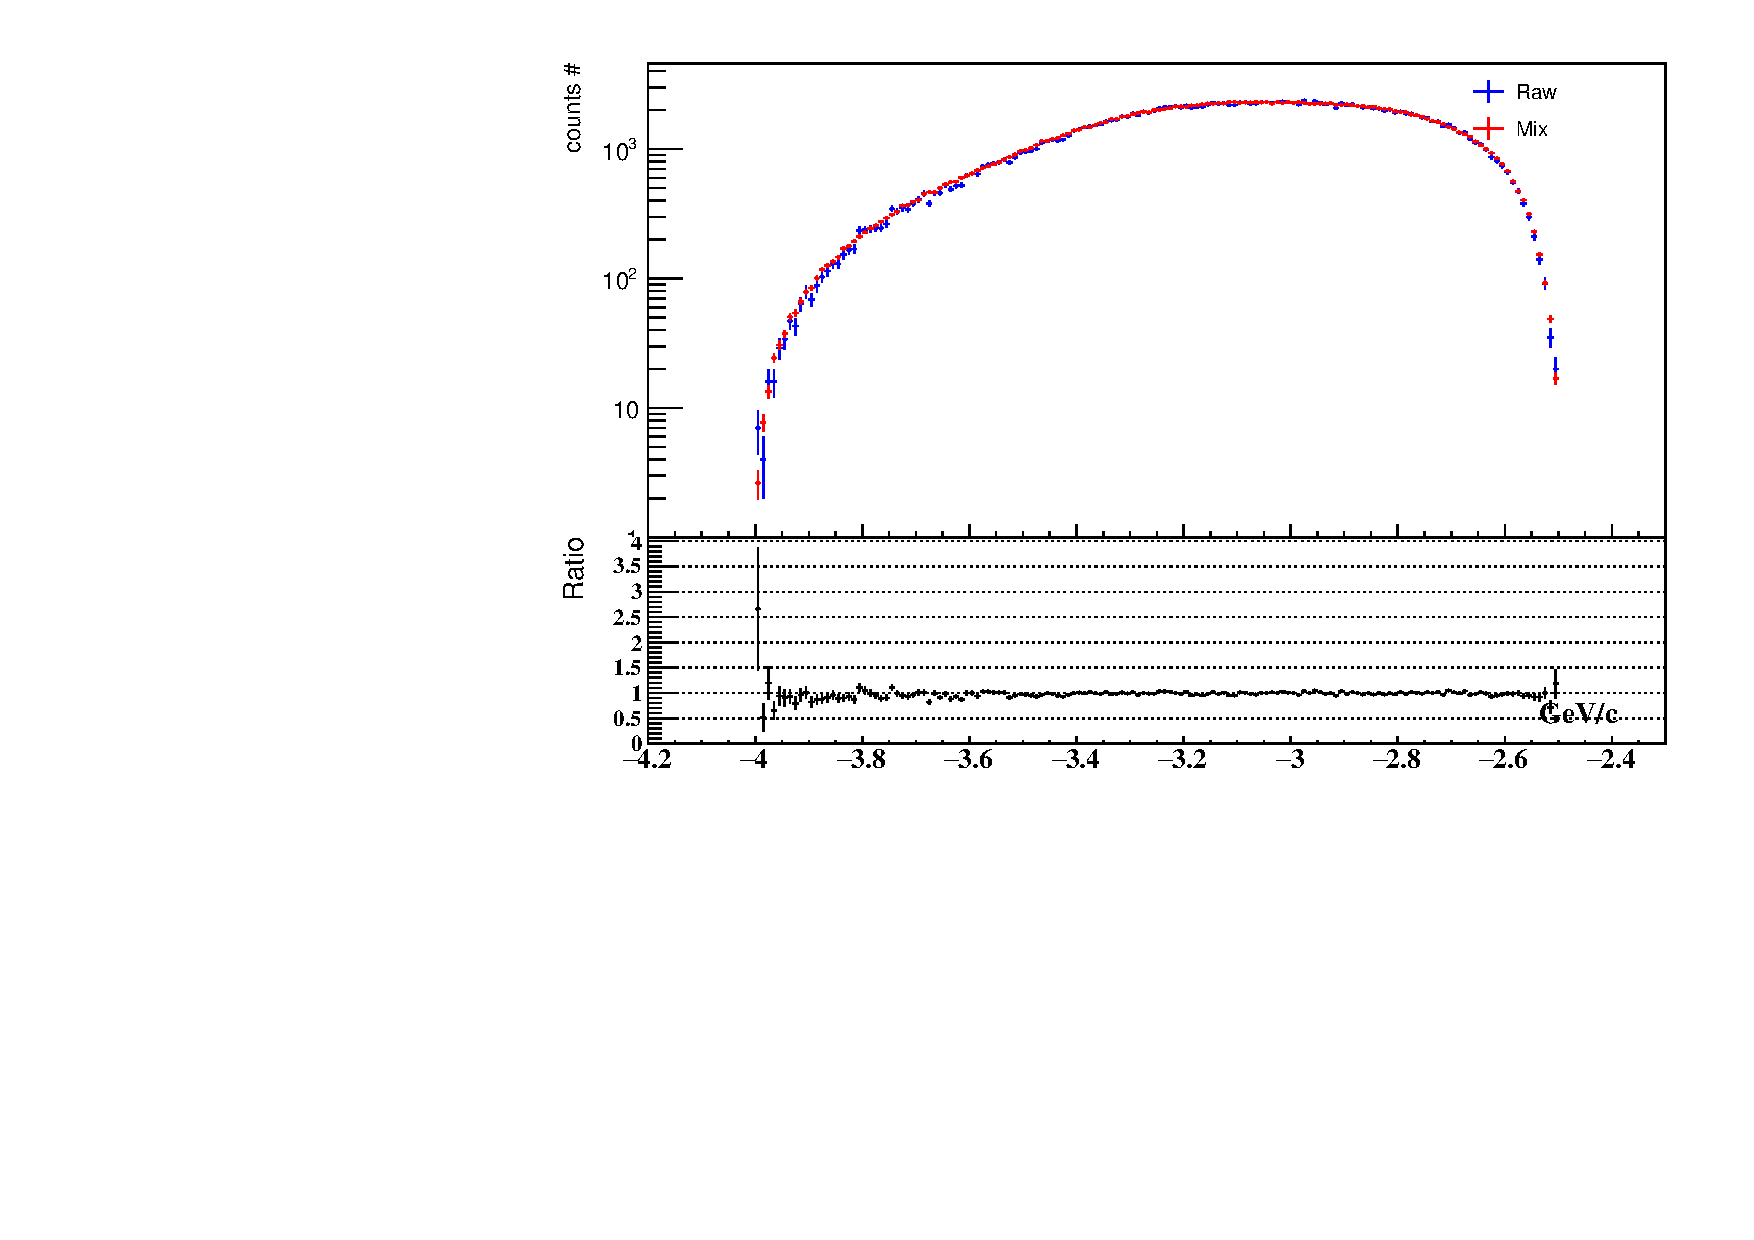
\includegraphics[width=5cm]{/Mixing/Y_MM.pdf}
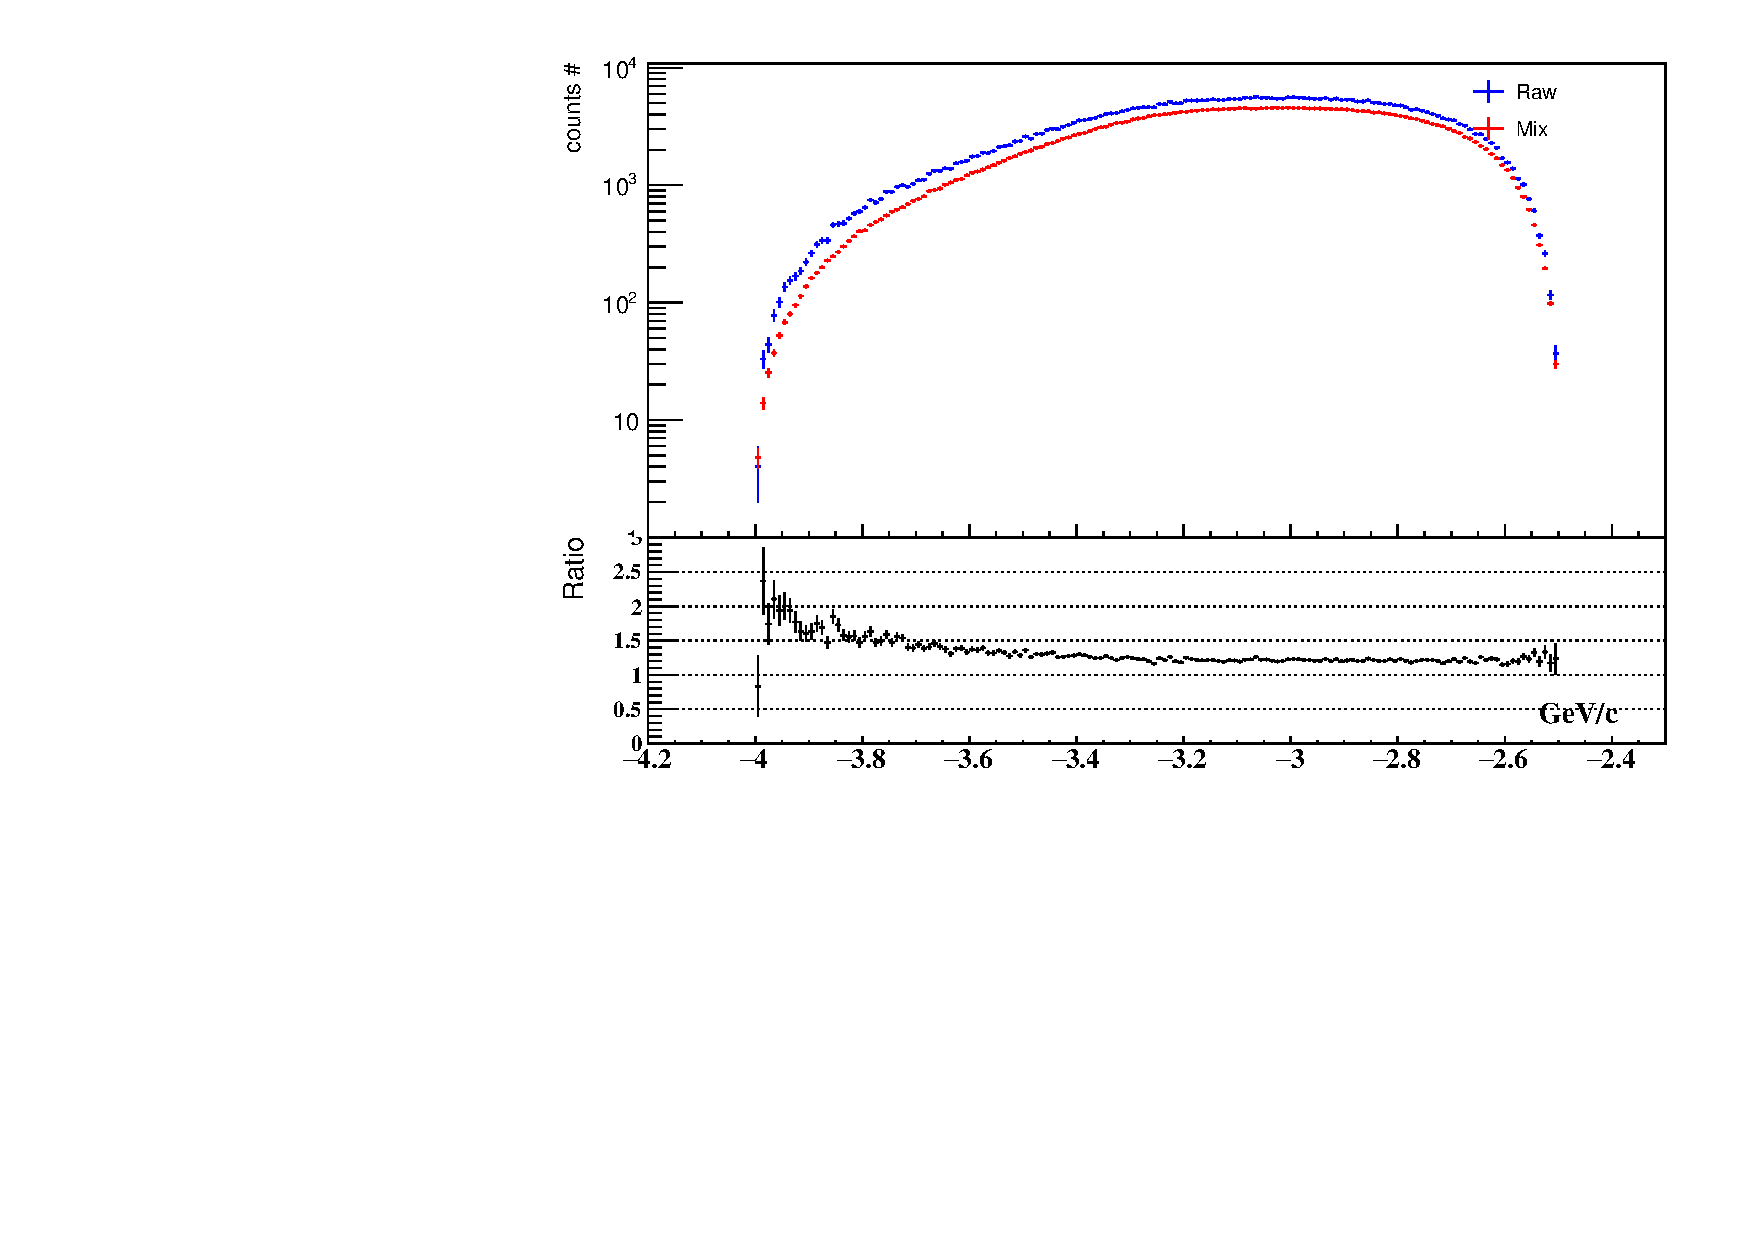
\includegraphics[width=5cm]{/Mixing/Y_PM.pdf}\\
\end{center}
\caption{\label{normalization}Comparison of raw and normalized mixed spectra as a function of invariant mass (top), \pt (center) and $y$ (bottom) for positive like sign dimuon (left), negative like sign dimuon (center) and unlike sign dimuon (right).}
\end{figure}

\begin{table}[!b]
  \centering
  \begin{tabular} { c | c | c | c}
    \hline
    centrality & $N^{\ups}$ &  \y & $N^{\ups}$ \\\hline
    0-10\% &  $ 393 \pm  41 \;(10.4\%) \pm  22 \;( 5.6\%) $   &  $[2.5-4]$ & $1107 \pm  70  \;( 6.3\%) \pm  43 \;( 3.9\%)$ \\
    10-30\% & $407 \pm  41 \;(10.1\%) \pm  21 \;( 5.1\%)$  & $[2.5-3]$ & $ 398 \pm 43 \;(10.8\%) \pm 17 \;(4.2\%) $ \\
    30-50\% & $ 218 \pm  34 \;(15.6\%) \pm  10 \;( 4.4\%) $ & $[3-3.5]$ & $ 548 \pm 48 \;(8.8\%) \pm 30 \;(5.4\%) $ \\
    50-90\% & $ 75 \pm  15 \;(20.0\%) \pm    3 \;( 4.5\%) $  & $[3.5-4]$ & $ 167 \pm 23 \;(13.7\%) \pm 11 \;(6.9\%) $ \\
    0-20\% & $ 603 \pm 50 \;(8.3\%) \pm 29 \;(4.9\%) $   &  & \\
    20-90\% & $ 506 \pm 46 \;(9.2\%) \pm 27 \;(5.4\%) $   &  & \\\hline
  \end{tabular}
  \caption{\label{NUps}\ups raw yield as a function of centrality classes and rapidity.} 
\end{table}

\paragraph{}
To conclude, 48 tests are performed for the integrated spectrum whereas 16 tests are performed for all other spectra.
The mean value over all the tests is taken as the number of extracted \ups as well as the mean value of the statistical uncertainties return by the fits on the integral of the signal function between 0 to 15 GeV/$c^2$.
The systematic uncertainty on the signal extraction is defined by the RMS of the distribution of tests shown in the figure \ref{systSignal}.
It has been checked that all the tests for all the intervals under study do not exceed 2 RMS.
All the results are reported in the table \ref{NUps}.
The systematic uncertainty varies between 4\% (integrated spectrum) to 7\% (most forward interval). 

\begin{figure}[!t]
\begin{center}
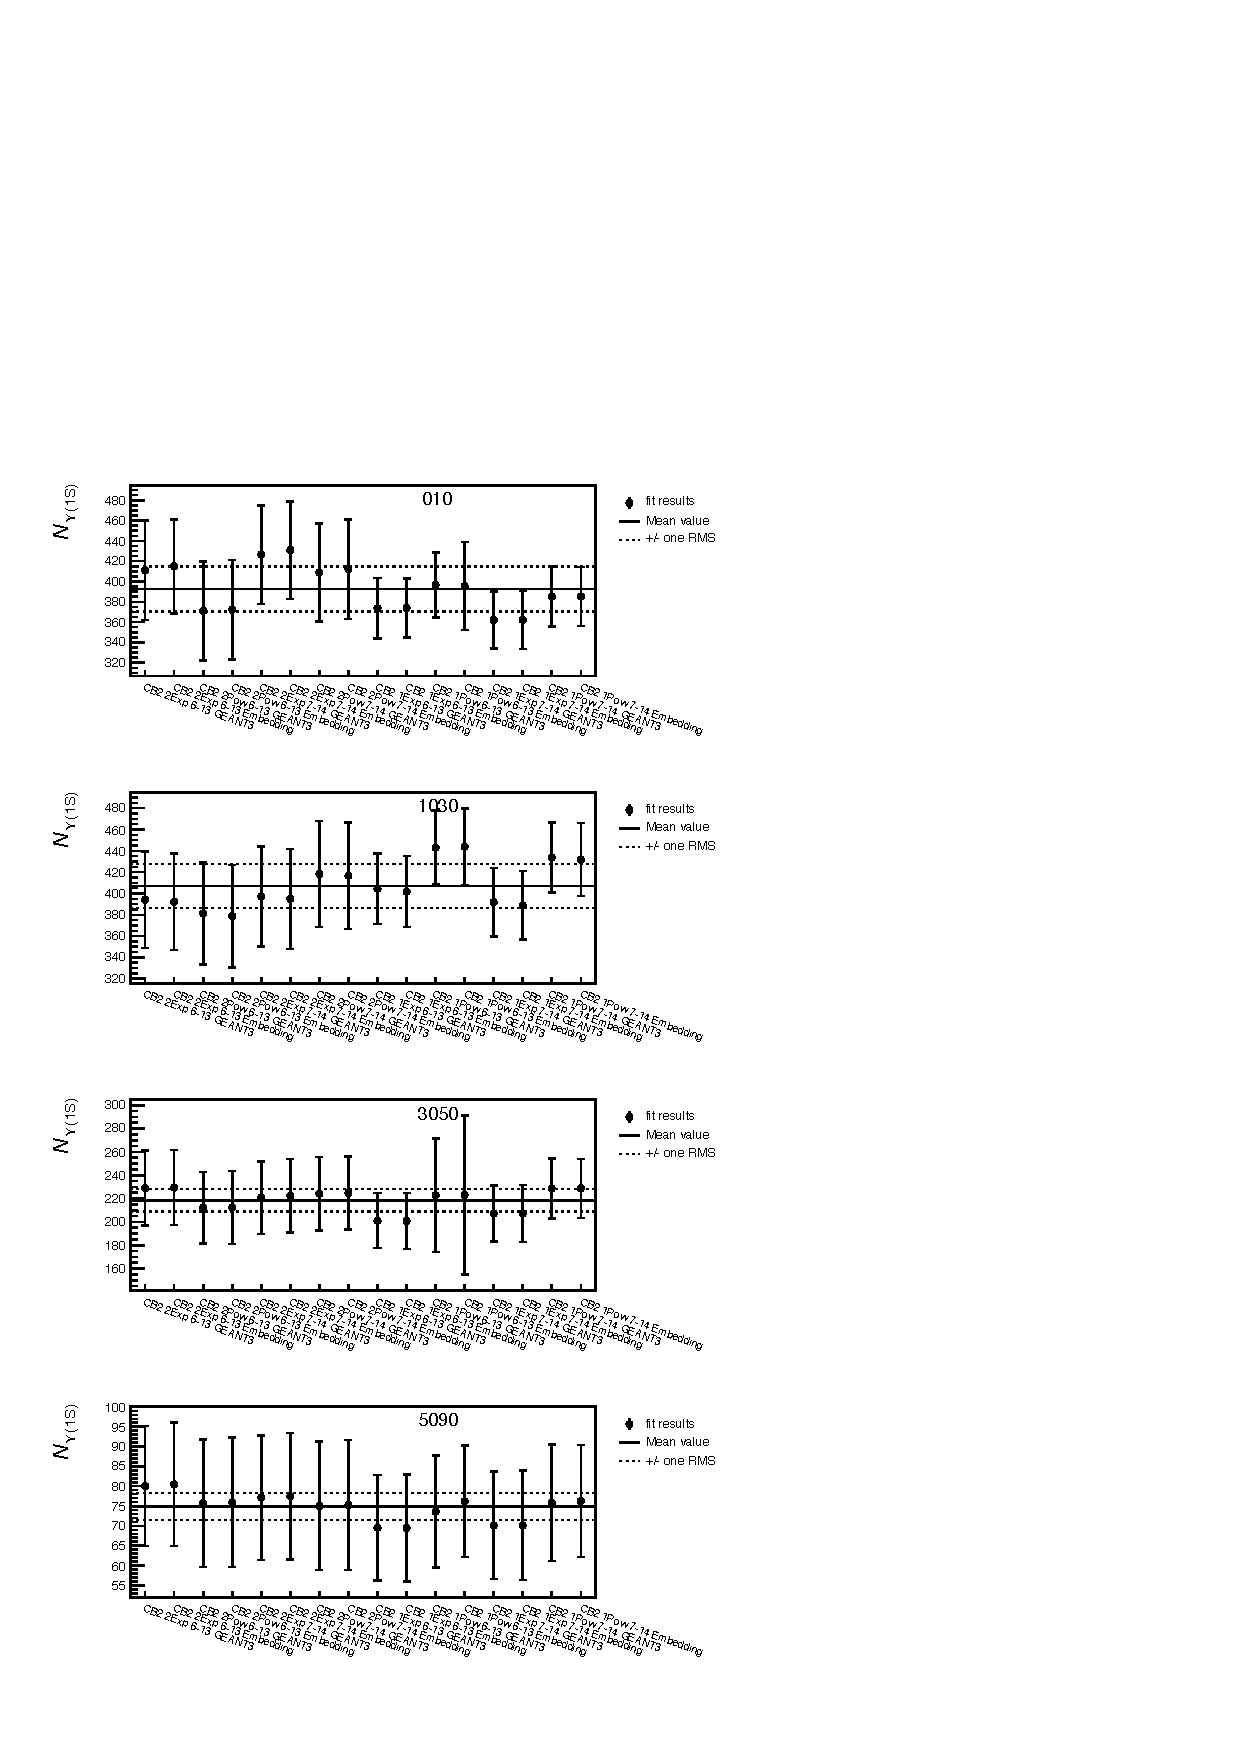
\includegraphics[width=6cm,height=9cm]{/Signal/sysYields_Cent.pdf}
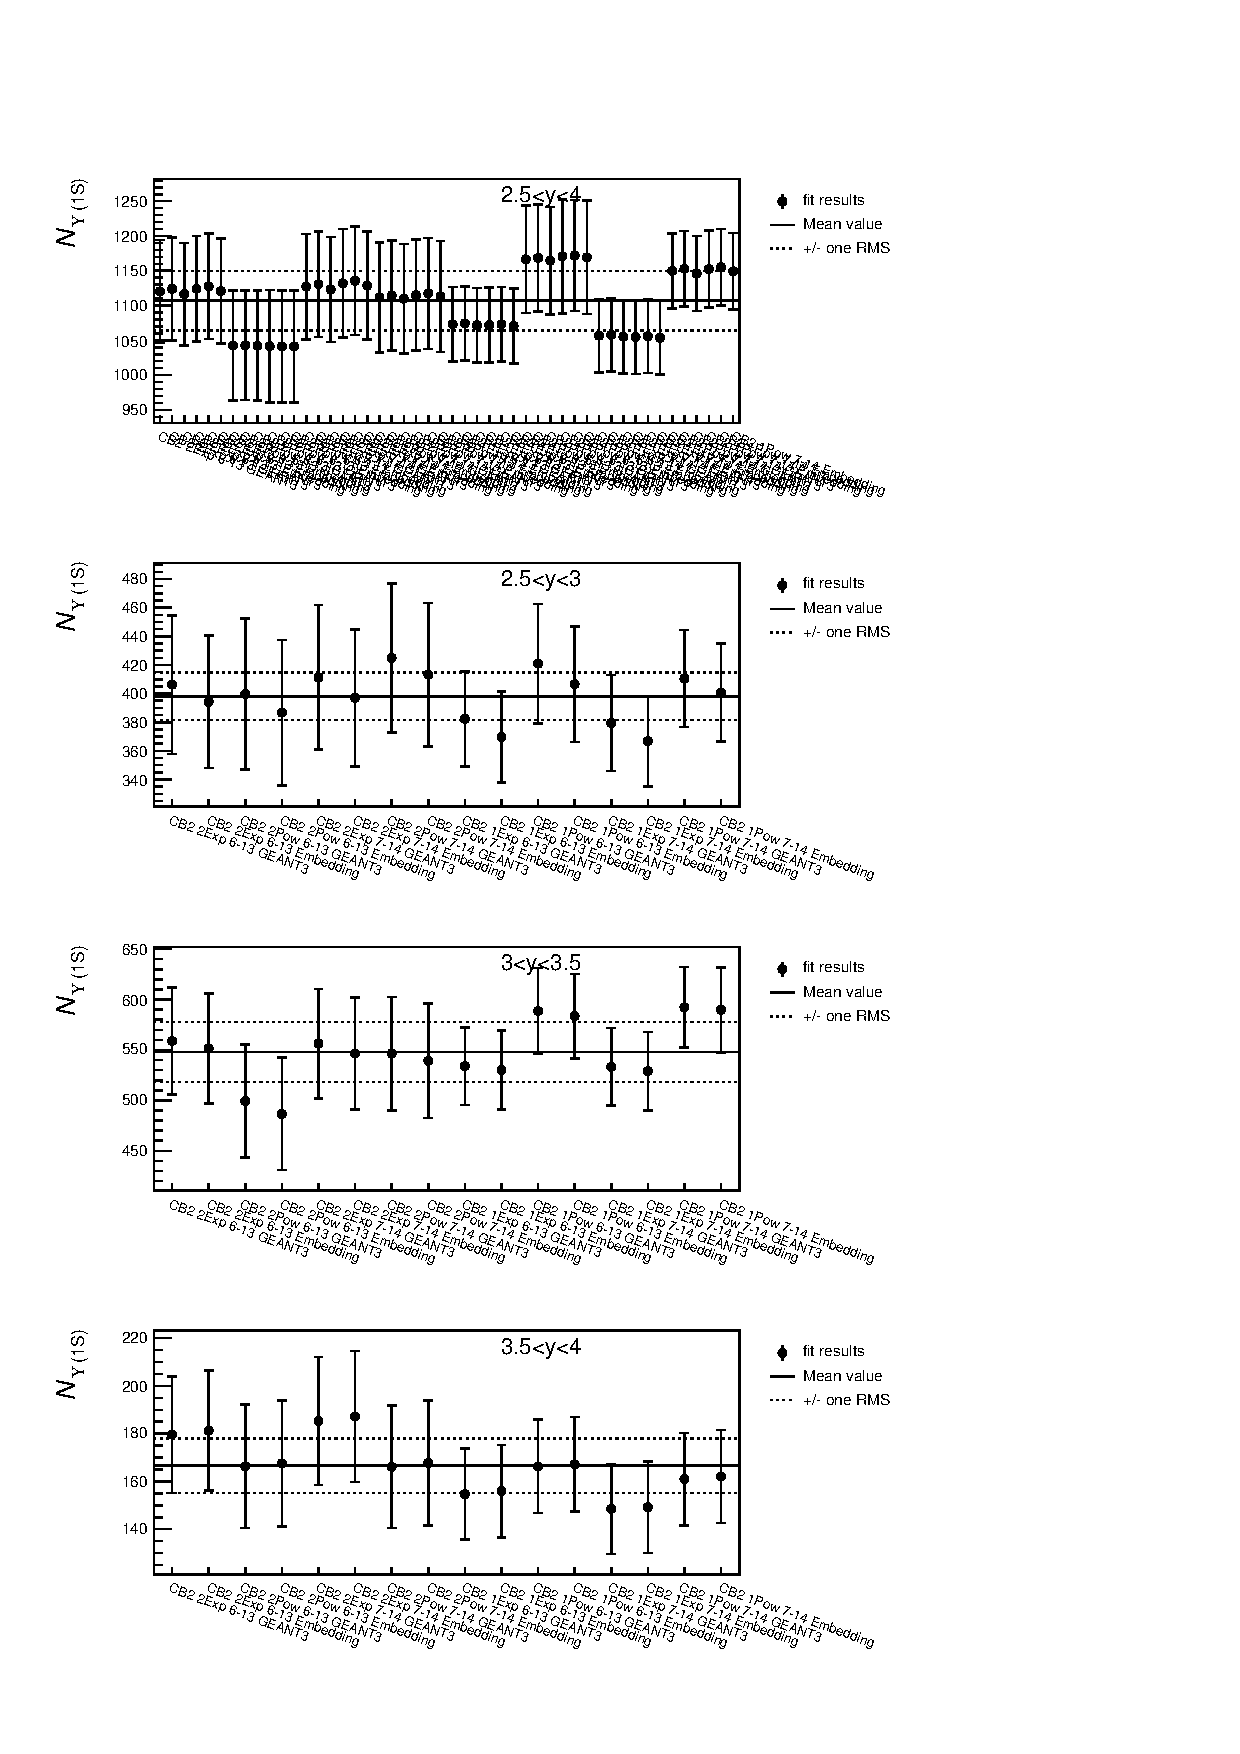
\includegraphics[width=6cm,height=9cm]{/Signal/sysYields_Y.pdf}
\end{center}
\caption{\label{systSignal}Number of measured \ups as a function of the different tests for the centrality classes (left) and integrated spectrum and rapidity intervals (right).}
\end{figure}




\subsection{MC systematic}

\begin{figure}[!b]
\begin{center}
  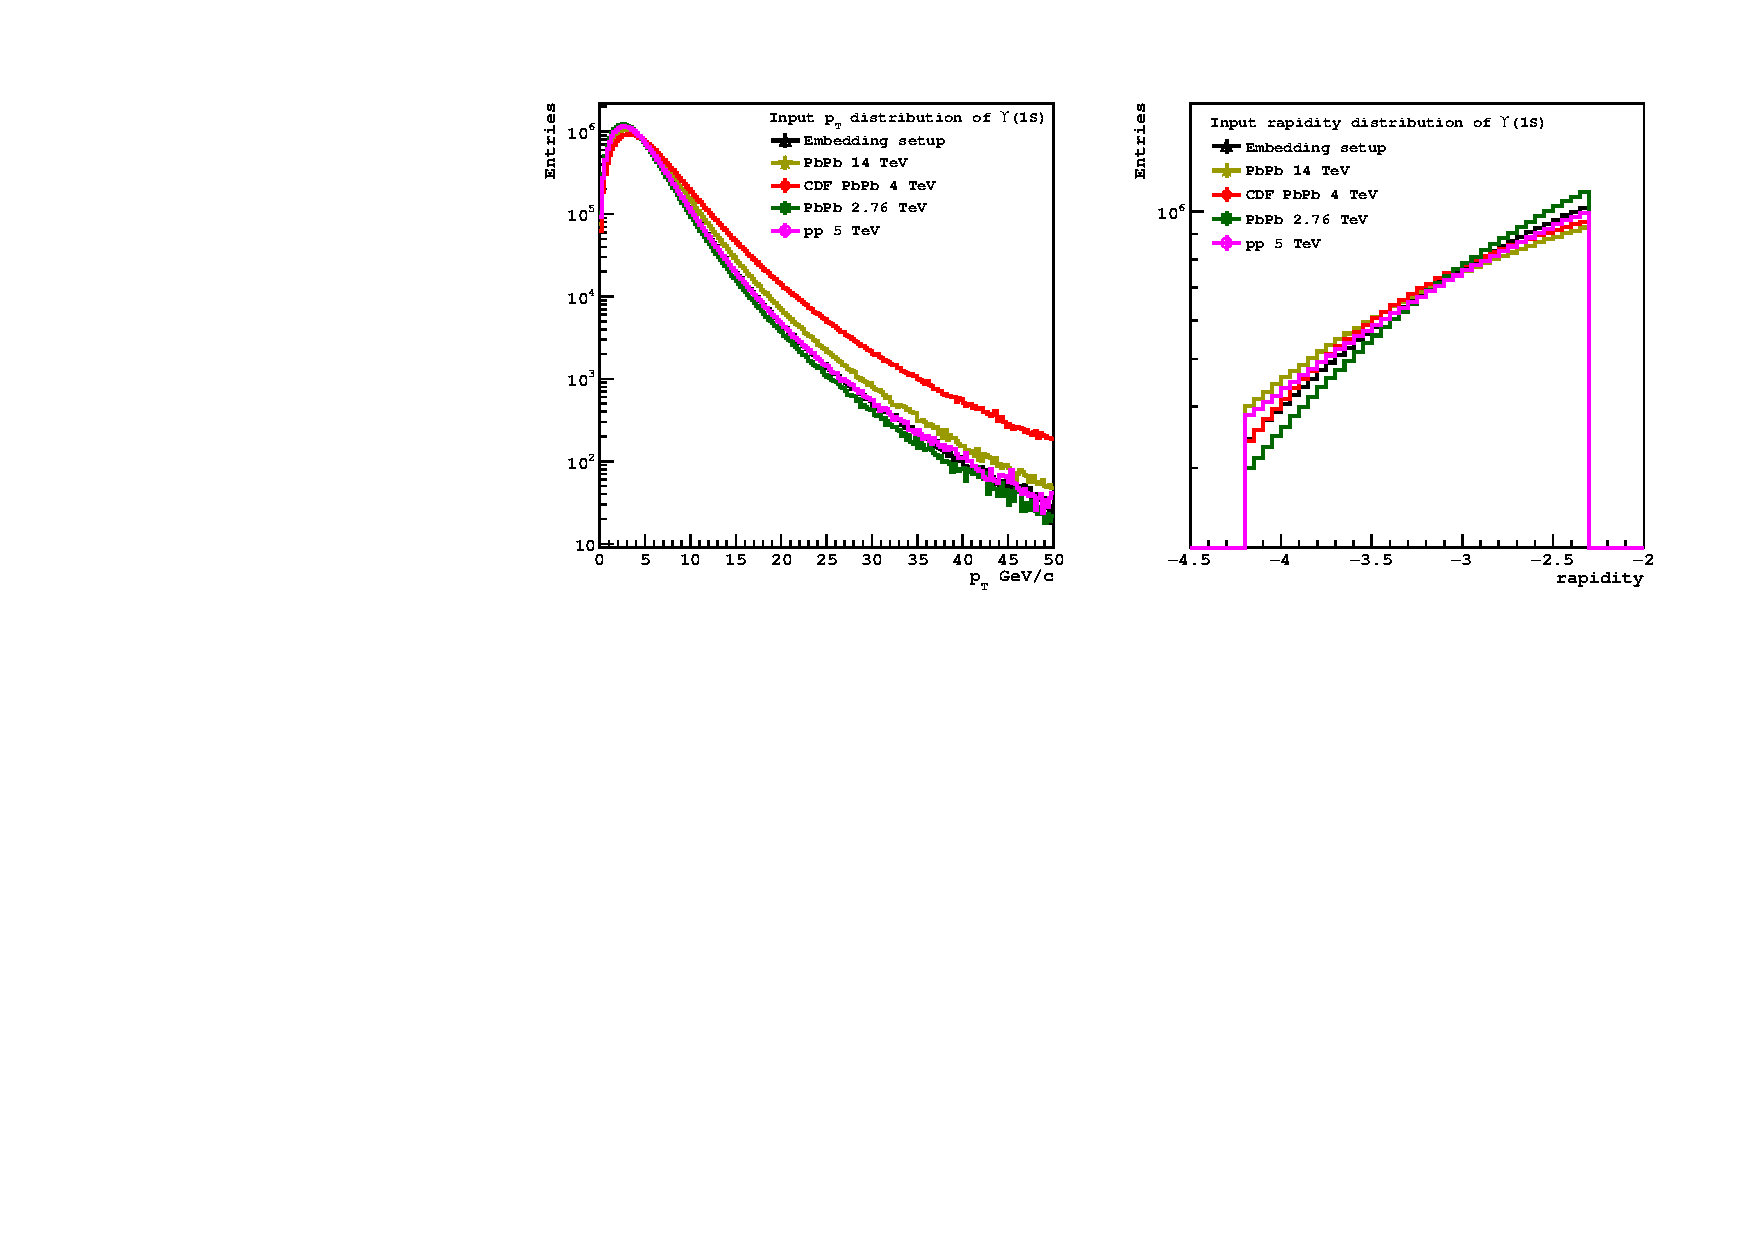
\includegraphics[width=13cm]{/Indra_MC_Upsi_Syst_2016_06_07/input_pt_rap_dist.pdf}
 \end{center} 
 \caption{\label{inputMC} Input \pt  and \y  distributions for different simultion setups.}
\end{figure}   

\paragraph{}
The MC productions like pure simulation or embedding are based on input \pt and \y distributions.
The parametrization used for both productions is defined as the product of the pp parametrization available in AliGenMuonLib class at 5 TeV times a shadowing parametrization at 2.76 TeV similar to EKS98.
In order to test the validity of this parameterization and determine a associated systematic uncertainty we have computed the \ups $A\epsilon$ correction from various kinematic shapes represented on the figure \ref{inputMC} such as: PbPb at 14 TeV, PbPb at 4 TeV extrapolated from CDF data, PbPb at 2.76 TeV and also a pp parameterization at 5 TeV.
Note that due to the small statistic available we can not apply a iterative data-driven method as in the \jpsi case.
The $A\epsilon$ results are shown as a function of the run number, \pt and \y on the figure \ref{sysinputMC}.
The maximum relative difference between the various input parametrization is taken as input MC systematic uncertainty and is $\sim1\%$ in the integrated case, almost flat and $\sim2\%$ as a function of \pt and a variation of 1-3\% is observed as a function of $y$.
The input MC systematic is correlated as a function of centrality and not as a function of \pt and $y$.
TBCompleted

\begin{figure}[!h]
\begin{center}
  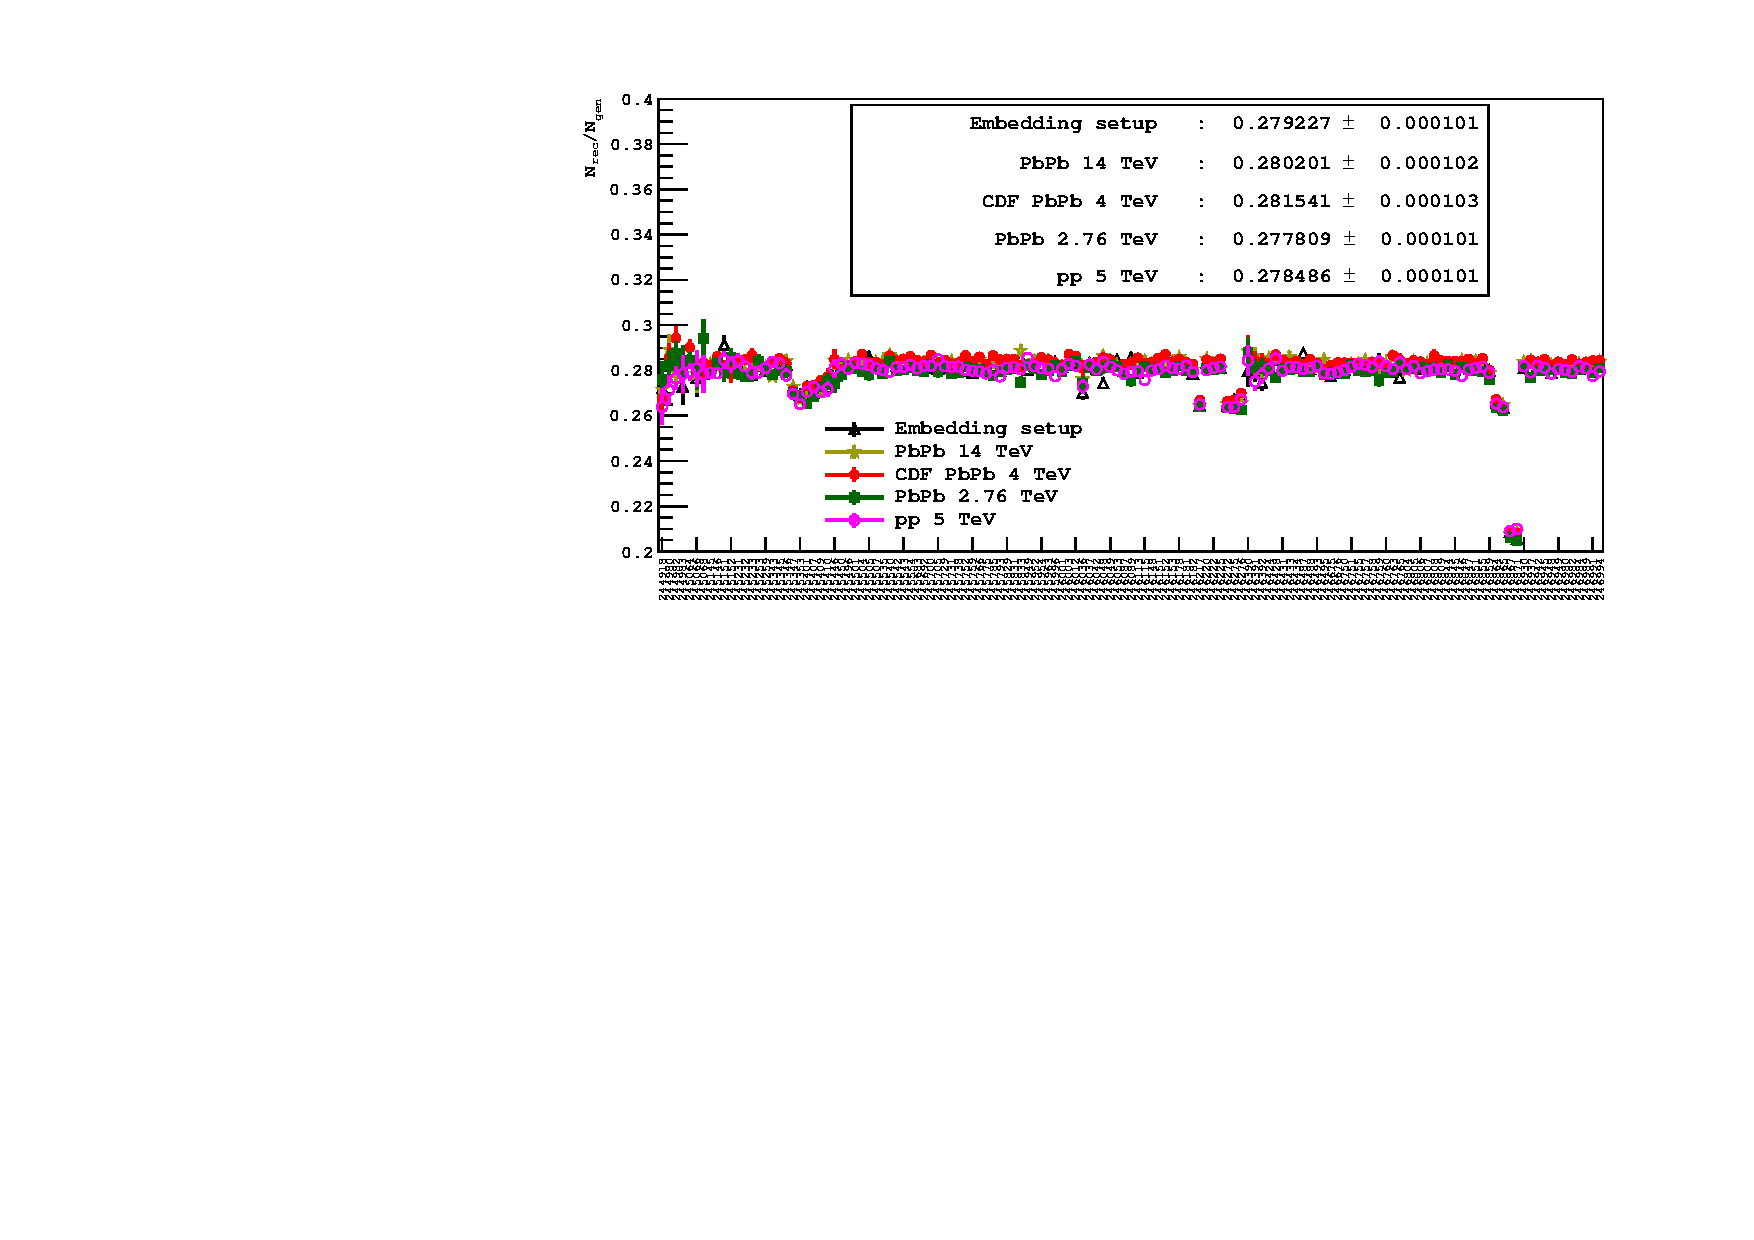
\includegraphics[width=13.cm,height=5.cm]{/Indra_MC_Upsi_Syst_2016_06_07/AxE_integrated.pdf}
  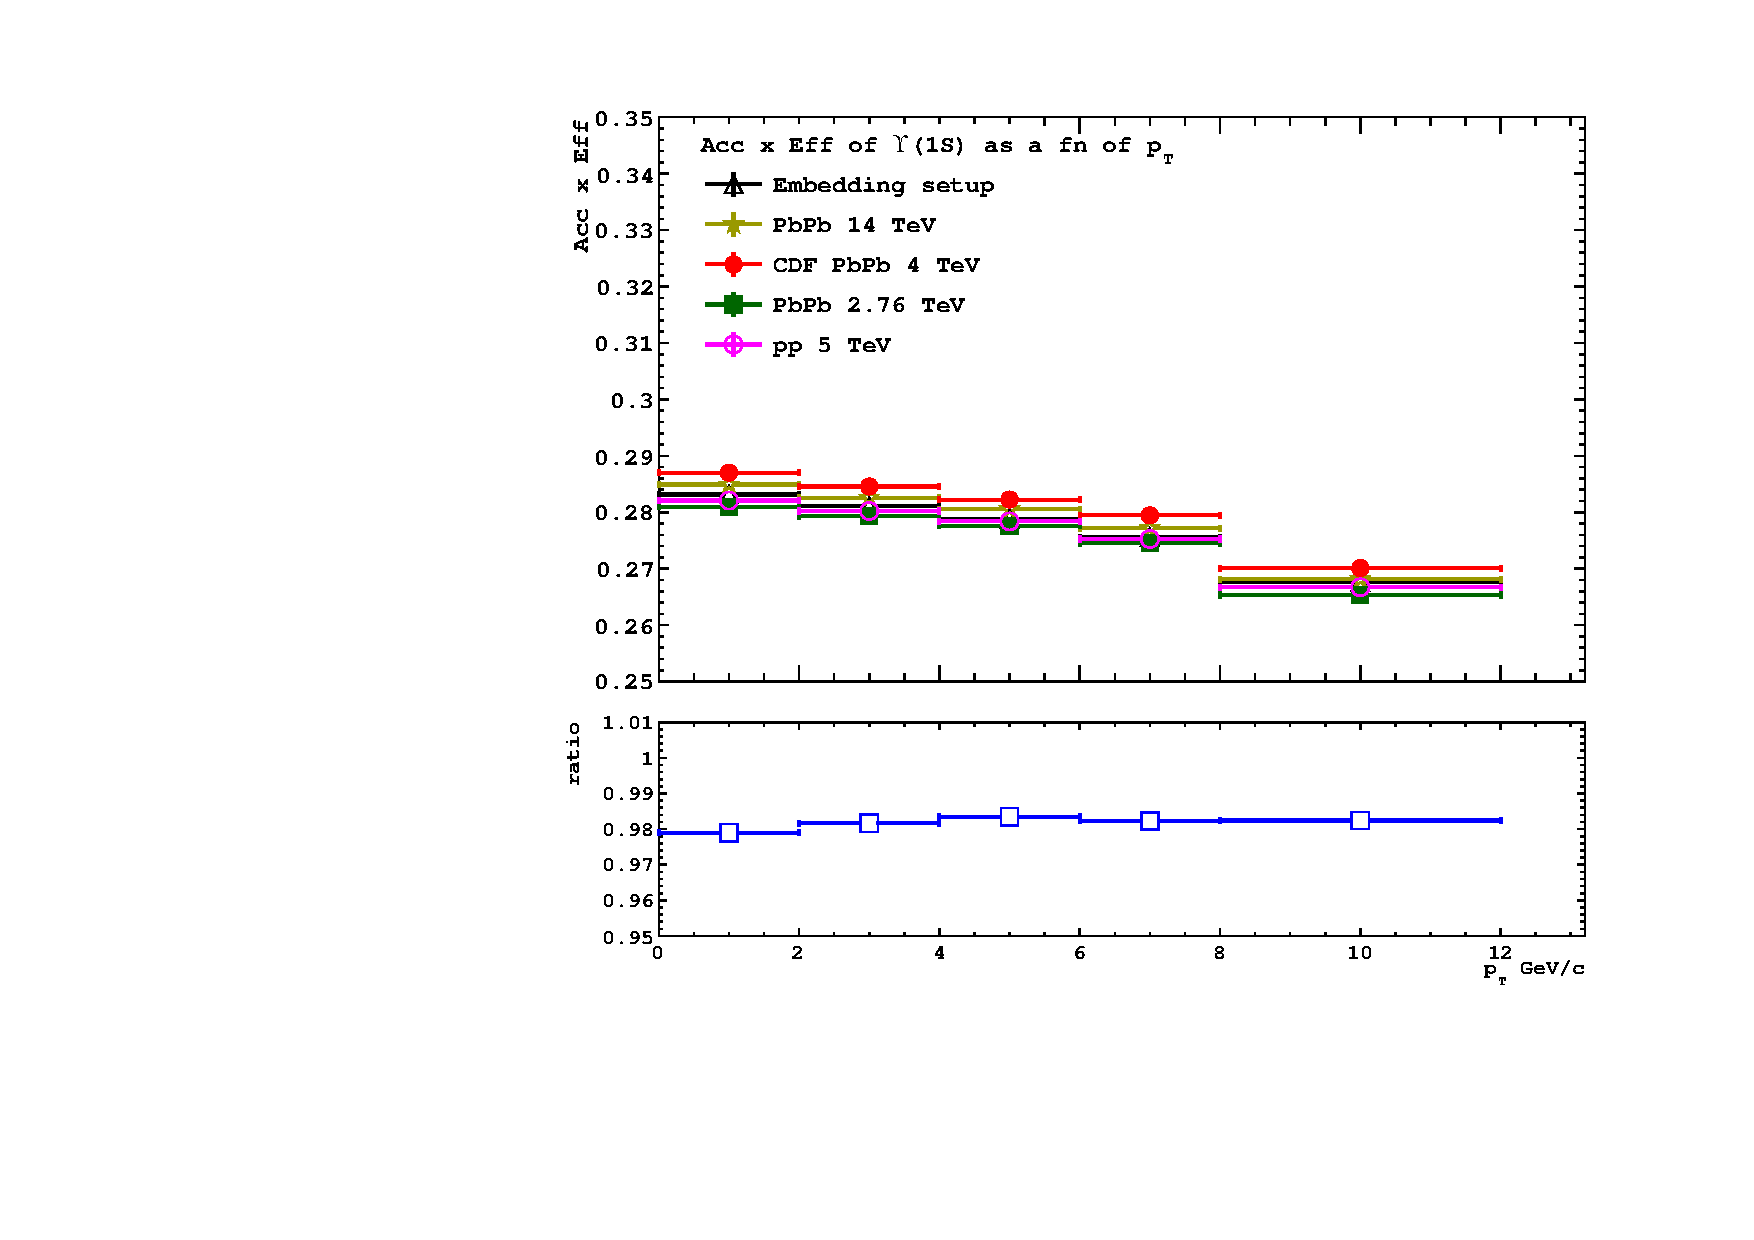
\includegraphics[width=6.5cm]{/Indra_MC_Upsi_Syst_2016_06_07/AxE_pt.pdf}
  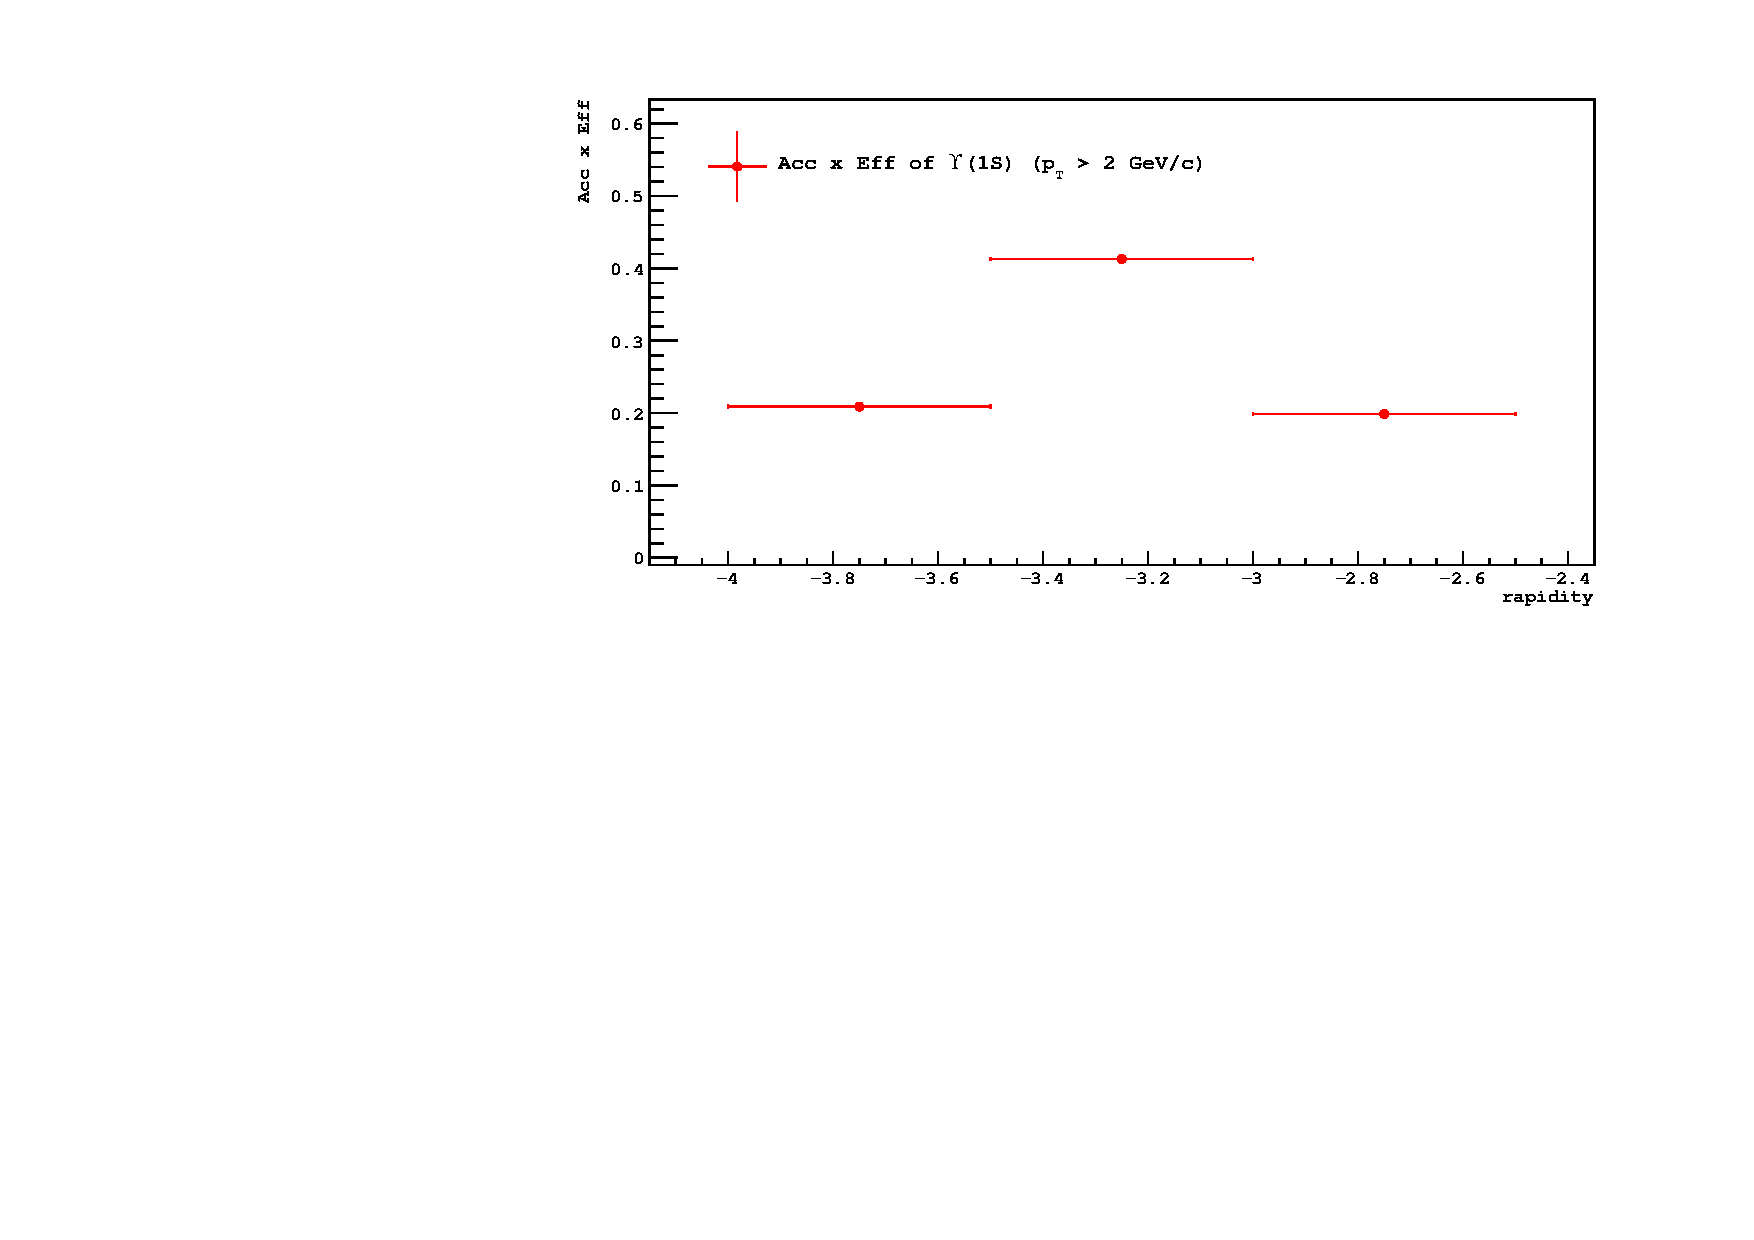
\includegraphics[width=6.5cm]{/Indra_MC_Upsi_Syst_2016_06_07/AxE_rap.pdf}
   \end{center} 
\caption{\label{sysinputMC} $A\epsilon$ as function of run numbers integrated over \pt and \y for different input parameterizations. The maximum relative difference of $100 \times(1-\frac{0.2778}{0.2815}) = 1.3 \% \sim 1\%$ is taken as MC systematics on integrated results.  (Results in earlier analysis on \upsi suppression in 2.76 TeV found 4\%)
In \pt and \y bins a variation of 1-3\% have been found. }
\end{figure}       





\subsection{Tracker systematic}

\paragraph{}
The determination of the tracking efficiency of the muon spectrometer and its systematic uncertainties are reported in details in the section 7 of the \jpsi analysis note (\href{https://aliceinfo.cern.ch/Notes/node/486}{here}) referring to the same Pb-Pb data sample (LHC15o period).
A 1.5\% systematics uncertainty is observed in average for single muons, with variations depending on the kinematics, the maximum being always with $2-3\sigma$.
This results in a 3\% systematics uncertainty for dimuons, considered as fully correlated as a function of centrality but not as a function of \pt and $y$.
Another source of uncertainty comes from the loss of tracking efficiency with increasing collision centrality, as the detector occupancy increases. 
This loss of efficiency is reproduced by embedding simulated \ups into real events as it could be observed on the figure \ref{AccEffplots}.
The differences in the efficiency drop between data and MC amount to $\sim0.5\%$ in most central collisions,
which results in a systematic uncertainty of $\sim1\%$ for \jpsi which should be even lower for \ups.
This uncertainty decreases with decreasing centrality, down to 0 in peripheral events, and is considered as fully correlated as a function of \pt and $y$.







\subsection{\label{systTrigger}Trigger systematics}

\paragraph{}
Three different sources of systematic uncertainties have been taken into account with respect to the muon trigger system:

\begin{itemize}
  \item the real trigger response is different with respect to the one used in Monte Carlo (MC) simulations;
  \item the efficiency values measured using real data are used as part of the MC input. Different methods can be used to evaluate the efficiency. Each method provides a slightly different efficiency value. The spreading of the possible values has to be evaluated;
  \item the $A\times\epsilon$ used within simulations can be altered by the efficiency evaluation method, as discussed in the previous point. The variation of $A\times\epsilon$ should be evaluated as well.
\end{itemize}

Each of these points should be considered in order to provide a comprehensive quotation of the overall systematic uncertainty.

\subsubsection{Trigger response}
The trigger Response Function (RF) is defined as in equation \ref{eq:RF}, where:
\begin{itemize}
	\item Lpt: Low $p_t$, $p_t>0.5 GeV/c$ cut;
	\item Apt: All $p_t$, no $p_t$ cut
\end{itemize}

\begin{equation}\label{eq:RF}
RF_{(MC,Data)}=\frac{N_{Lpt_{(MC,Data)}}}{N_{Apt_{(MC,Data)}}}	
\end{equation}

The trigger response observed in real events is different from the one measured in reconstructed MC events: the modeled response of the trigger system has some discrepancy with respect to the real one that cannot be easily represented within the MC detector parametrization. For this reason a correction has to be computed, in order to determine the magnitude of the induced systematic uncertainty.

The $RF_{Data}$ has been obtained using the full Pb-Pb $\sqrt{S_{NN}}=5.02 TeV$ data sample, while the $RF_{MC}$ has been computed analyzing a simulated data sample 10 times greater, in order to limit statistical uncertainties.
The RF should be studied with respect to $p_t$ and pseudo-rapidity ($\eta$). If studied with respect to $p_t$ the RF grows asymptotically to the unity by construction, while the knee of the trend is expected to be centered on the Lpt threshold of $p_t=0.5 GeV/c$.

\paragraph{Rescaling procedure}
The RF expresses the ratio between the number of Lpt and Apt matches. Since analyzing MC simulation only the $Apt_{MC}$ count is unbiased by the modeled trigger response, the corrected number of $Lpt_{MC}$ matches can be obtained as expressed in equation \ref{eq:correction}.

\begin{equation}\label{eq:correction}
	N_{\text{corrected $Lpt_{MC}$ with $RF_{(MC,Data)}$}}=N_{Apt_{MC}}\cdot RF_{(MC,Data)}
\end{equation}

This rescaling allows to obtain a corrected number of $Lpt_{MC}$.

\paragraph{Operational choices}
In order to obtain a precise result the RF can be evaluated with different levels of granularity. Instead of obtaining one $RF(p_t)$ integrated in rapidity we have divided the rapidity range in 10 sub-ranges. In such a way the $RF(p_t)$ becomes $RF(p_t; \eta)$. The obtained $RF(p_t; \eta)$ for respectively real data and MC simulations are represente in figures \ref{fig:RFRapidityData} and \ref{fig:RFRapidityMC}.

\begin{figure}[!h]
\begin{center}
  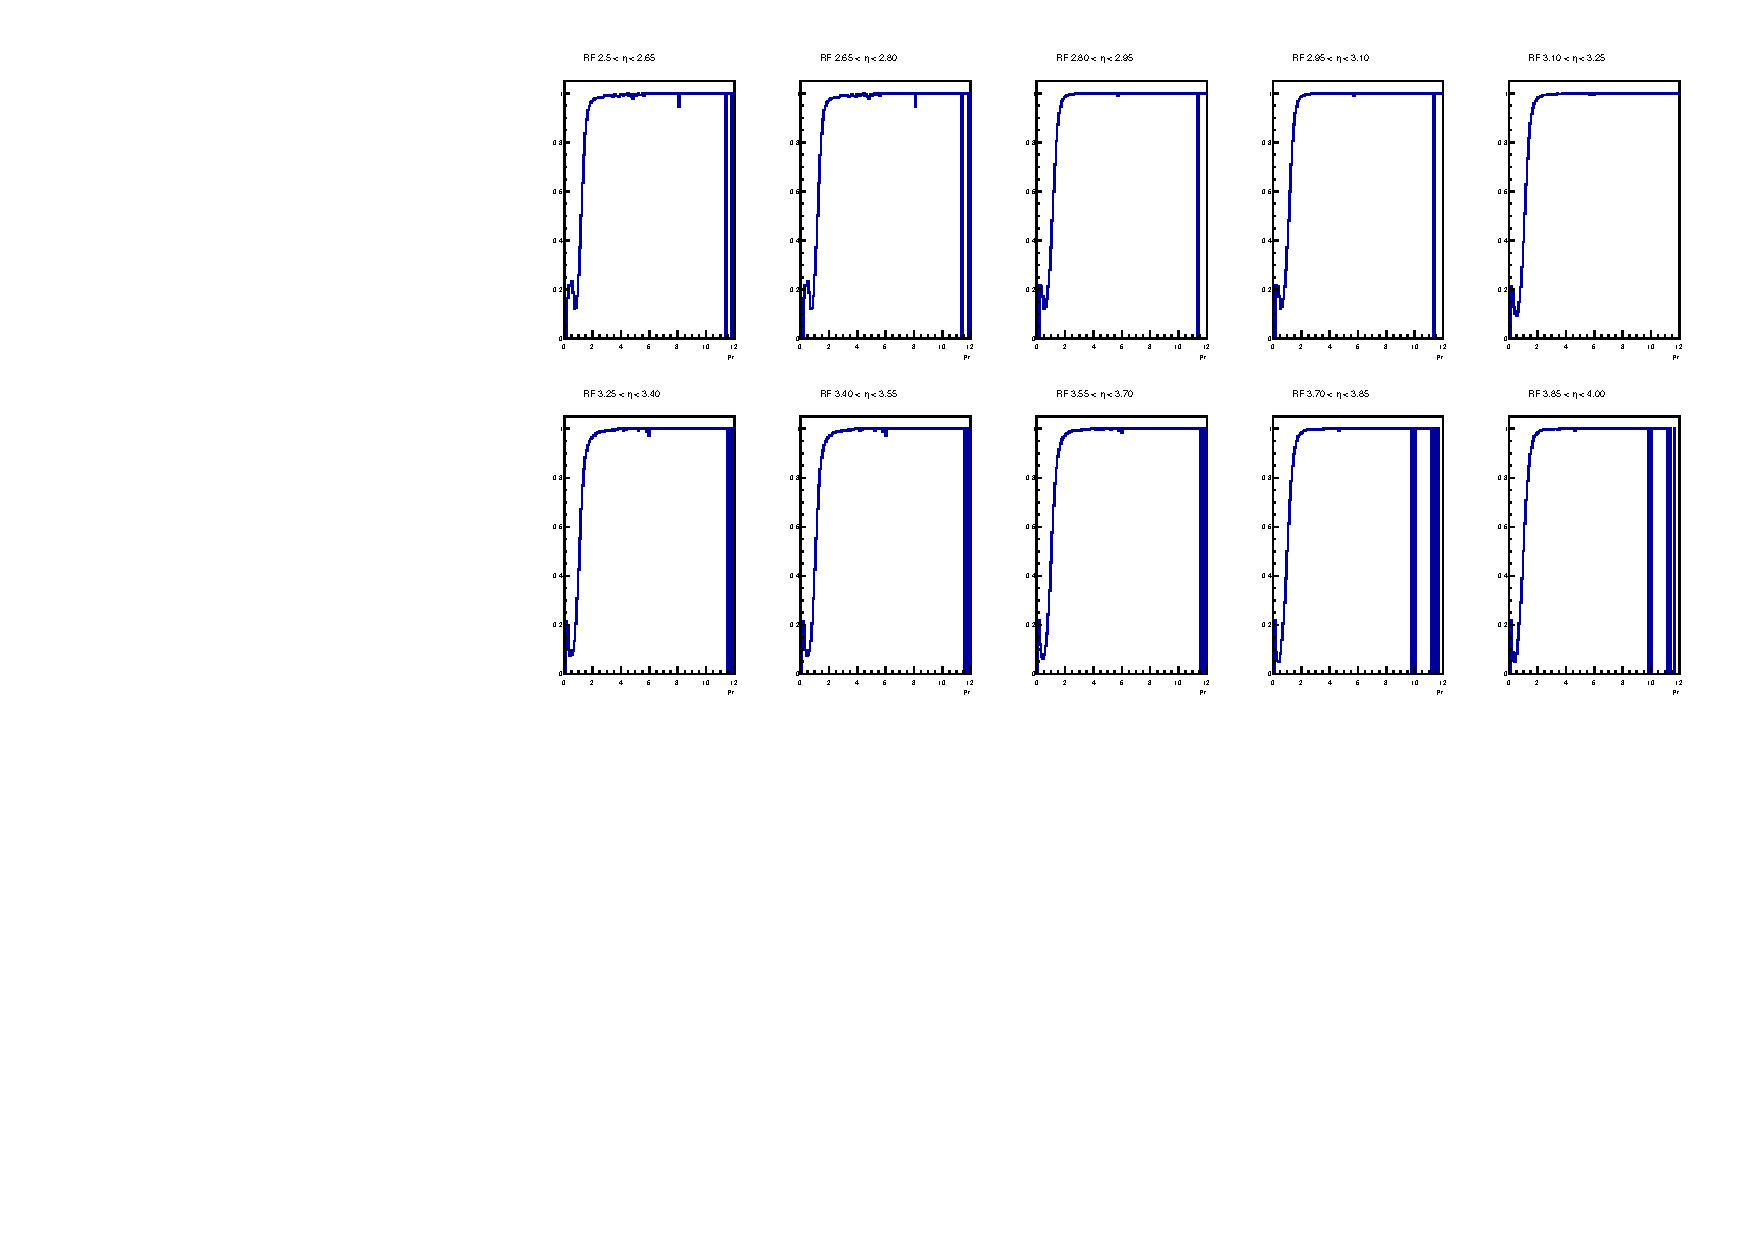
\includegraphics[width=13.cm,height=5.cm]{/Trigger/10_Rap_Bins_rebin8.pdf}
\end{center} 
\caption{\label{fig:RFRapidityData} Response functions of the muon trigger measured in real data. The RF has been obtained separately for 10 rapidity bins from $\eta=2.5$ to $\eta=4.0$}
\end{figure}  

\begin{figure}[!h]
\begin{center}
  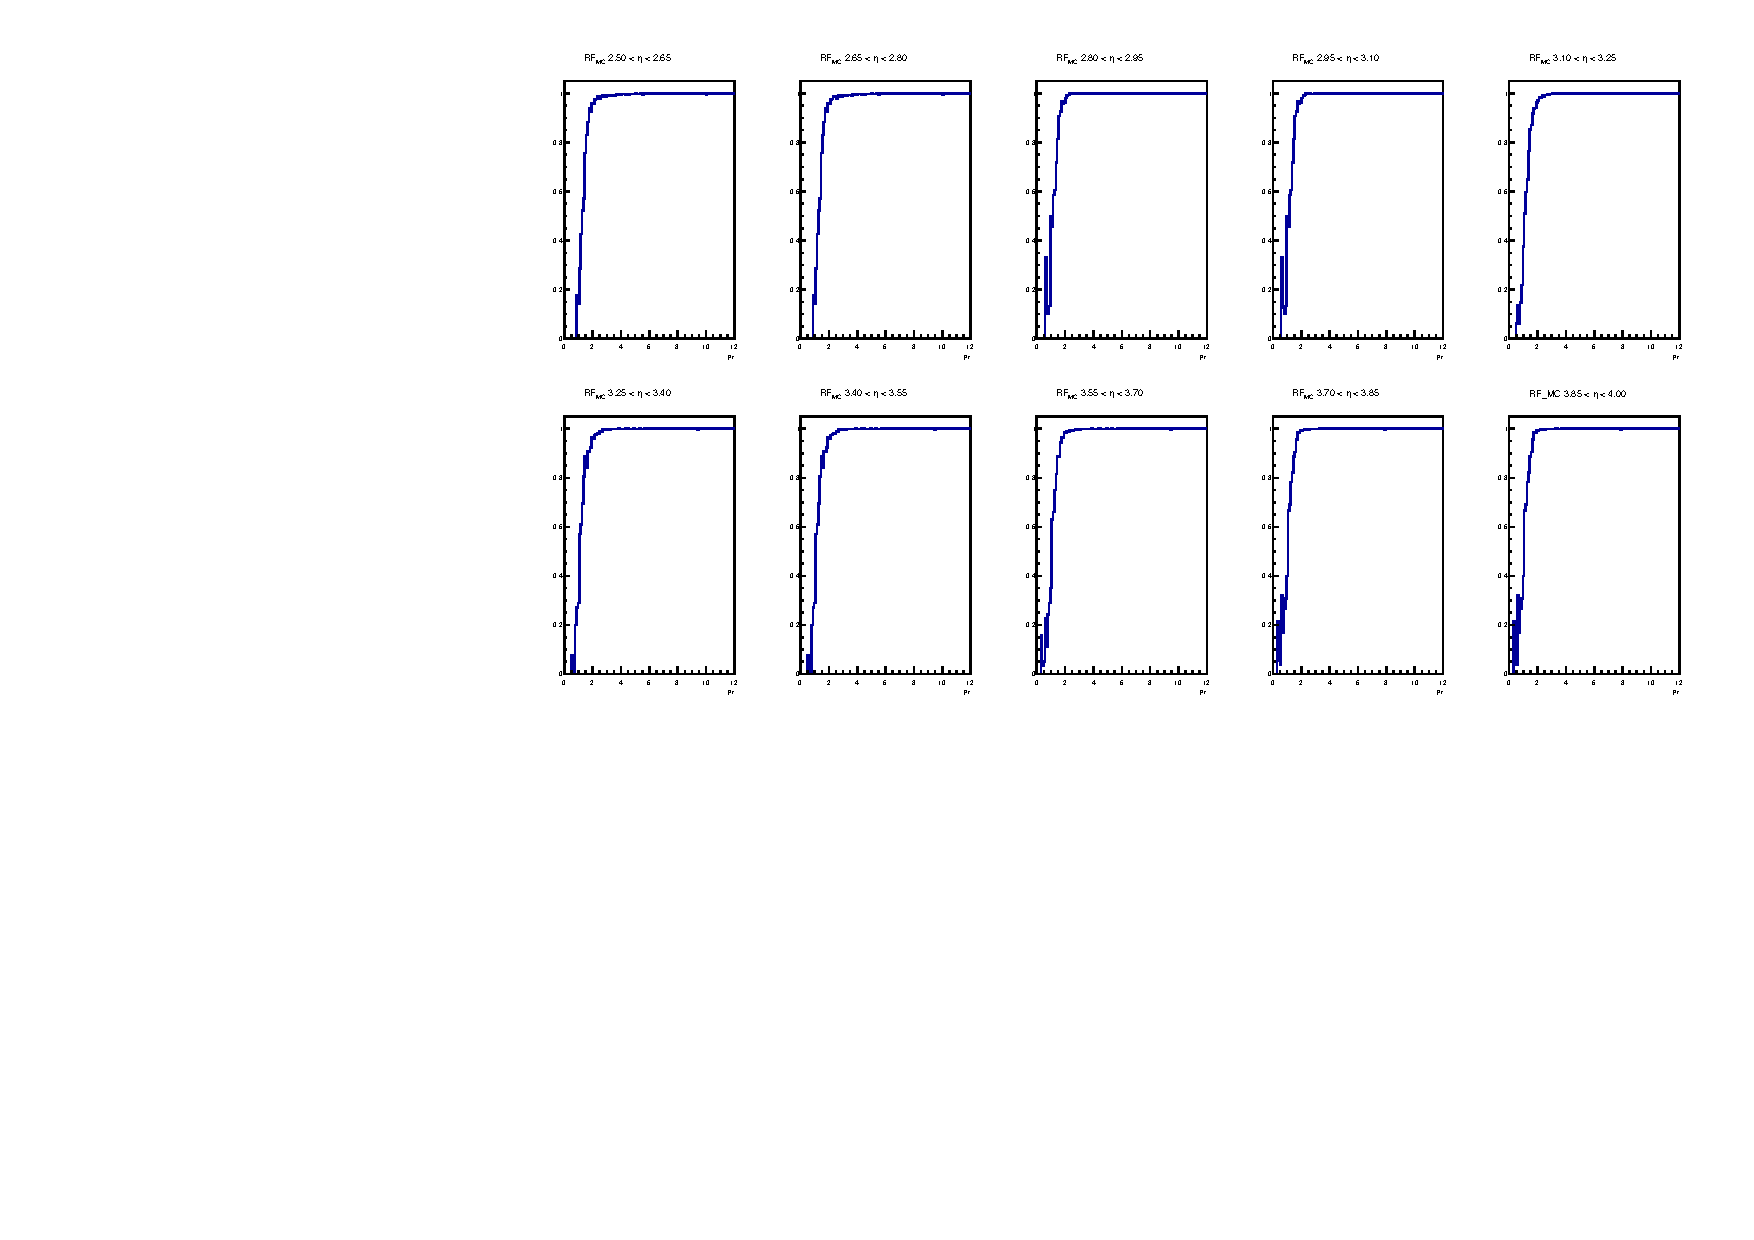
\includegraphics[width=13.cm,height=5.cm]{/Trigger/10_Rap_Bins_rebin8_MC.pdf}
\end{center} 
\caption{\label{fig:RFRapidityMC} Response functions of the muon trigger measured in reconstructed MC simulations. The RF has been obtained separately for 10 rapidity bins from $\eta=2.5$ to $\eta=4.0$}
\end{figure} 

The RF can be treated in two different ways, which converge in case of high statistics:
\begin{itemize}
	\item the RF is a functional form obtained via fitting the $\frac{Lpt}{Apt}$ histogram. This method can interpolate points in order to solve holes in the distribution, but has the drawback that the analytic form of the RF is not defined \textit{a priori};
	\item the $\frac{Lpt}{Apt}$ histogram per bin content can be directly used as the required weight, avoiding the fitting procedures and related NLO uncertainties. This method can't anyway be used in case of low statistics, since in that case fluctuations and holes risk to provide wrong weights to some of the entries.
\end{itemize} 
Both approaches have been pursued. The results are compatible within uncertainties, hence the direct use of histograms has been chosen as the adopted approach since is simpler. As seen in figure \ref{fig:RFRapidityData} some RFs present some holes at high $p_t$: this is mainly due to low statistics, but since by construction the RF converges at 1 for high $p_t$ the holes have been set to 1.

\paragraph{Entries weighting procedure}
Each entry of an invariant mass spectrum is the invariant mass of a pair of track identified as muons. Usually the di-particle invariant mass spectrum is obtained requiring each track to match Lpt condition. In order to apply any RF, and simulate the induced spectrum, the Apt request is instead applied to each track. The invariant mass spectrum is then obtained by assigning a weight to every track pair. The weight is computed for each pair using the previously evaluated ratio between Lpt and Apt matches (namely the RF). The weight is the product of the two RFs values obtained for each of the two paired tracks, as expressed in \ref{eq:weight}, where $p_{t1}$ and $\eta_{1}$ are the values of the first track composing the pair and $p_{t2}$ and $\eta_{2}$ are the values of the second.

\begin{equation}\label{eq:weight}
	weight_{(MC,Data)}(p_{t1},p_{t2};\eta_{1},\eta_{t2})=RF_{(MC,Data)}(p_{t1};\eta_{1})\cdot RF_{(MC,Data)}(p_{t2};\eta_{2})
\end{equation}

\paragraph{Systematic uncertainty evaluation}
In order to cope with the analysis choices the spectrometer rapidity acceptance range (2.5<y<4.0) has been divided in three rapidity region. One invariant mass spectrum has been computed for each region. The rapidity binning refers to the track pair rapidity.
The weighting procedure has been applied using both MC and Data weights, obtaining two invariant mass spectra for each track pair rapidity bin, hence for each rapidity bin two invariant mass spectra have been computed. The systematic uncertainty has been evaluated as the relative difference of the integral of the two spectra, as reported in \ref{eq:reldiff}, where $f_{MC}$ and $f_{Data}$ are the invariant mass spectra corrected using respectively $weight_{(MC)}$ and $weight_{(Data)}$.

\begin{equation}\label{eq:reldiff}
	Syst_{RF}=\frac{\abs{\int{f_{MC}(m)dm}-\int{f_{Data}(m)dm}}}{\int{f_{Data}(m)dm}}
\end{equation}

\paragraph{Results}
In figure \ref{fig:RFSyst} results are reported. Note that the statistical errors must not be considered as part of the systematic uncertainty since the two integrals of which the relative difference has been computed are based on the same data sample and so are totally correlated.

\begin{figure}[!h]
\begin{center}
  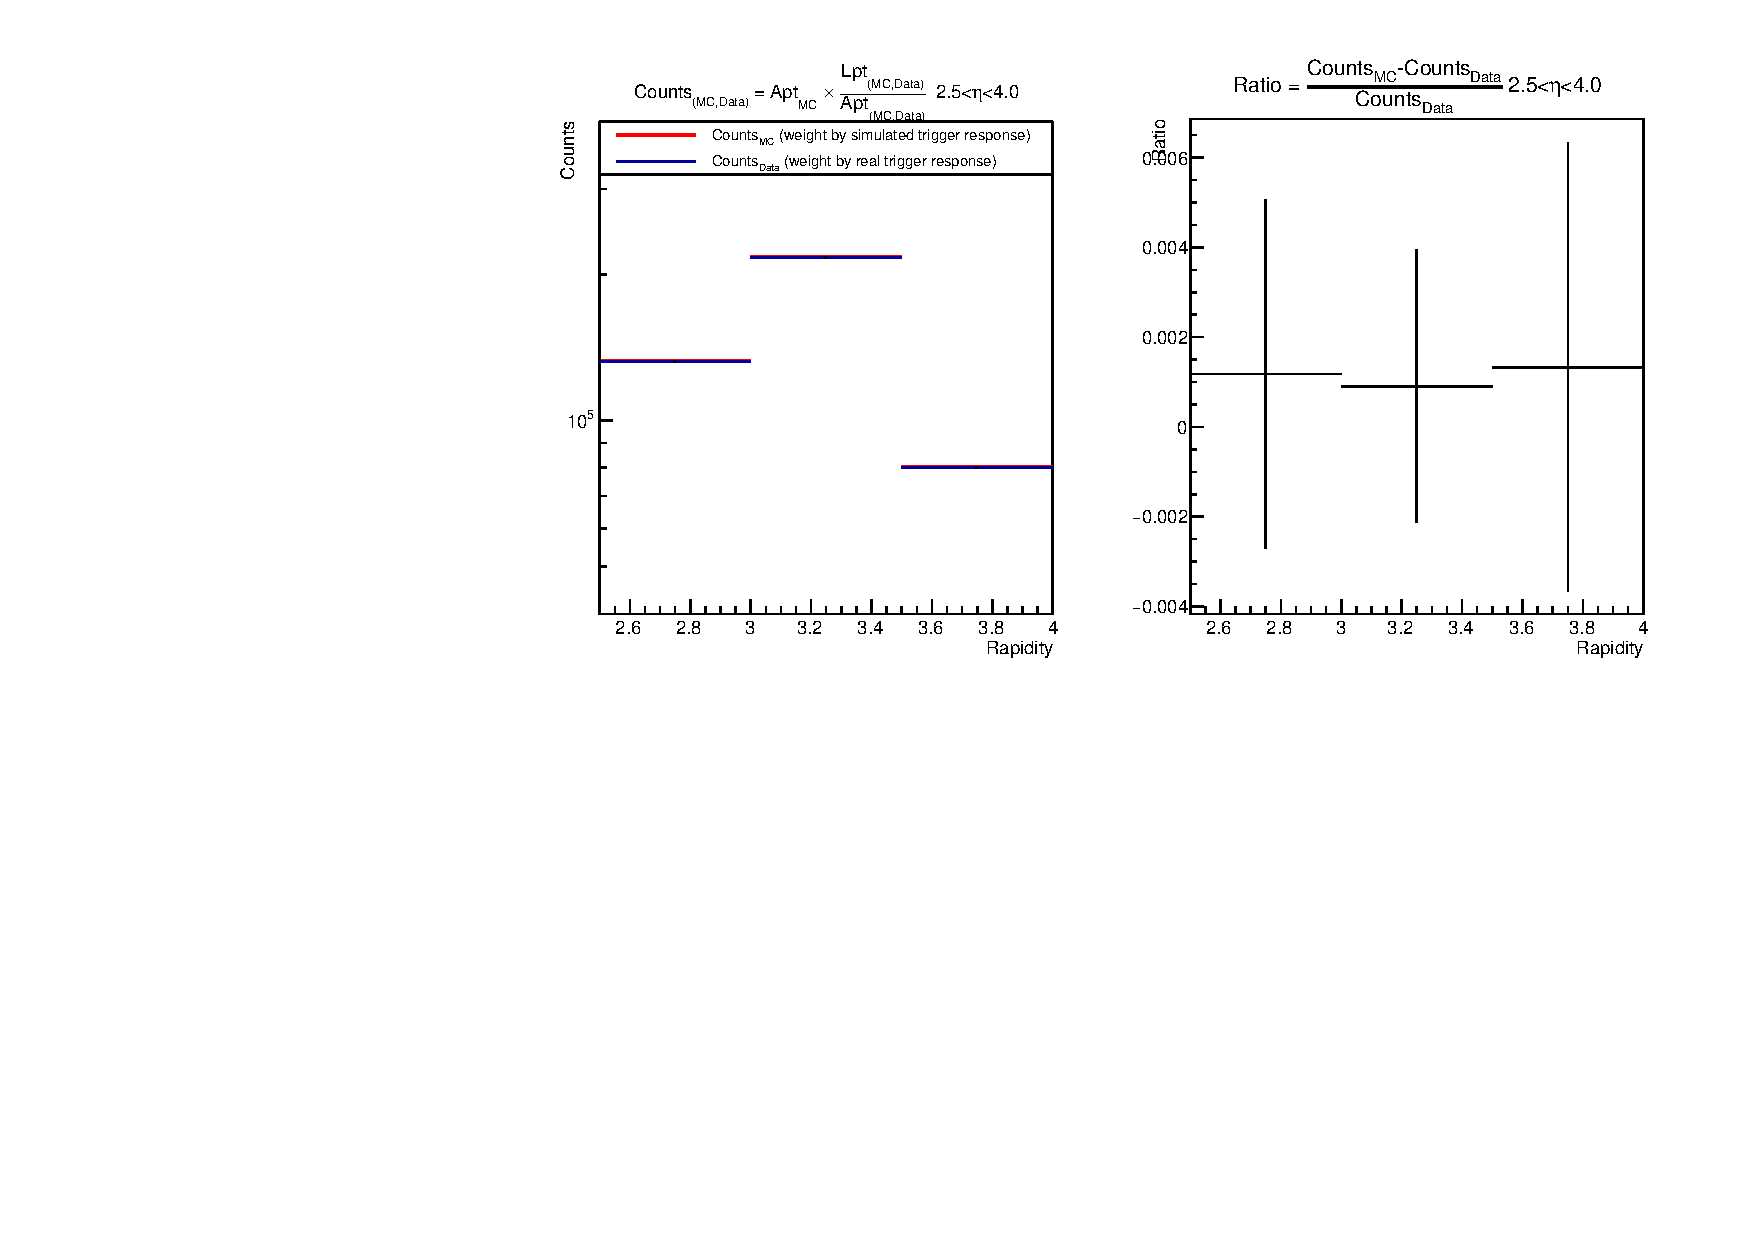
\includegraphics[width=13.cm]{/Trigger/ResponseFunctionSyst.pdf}
\end{center} 
\caption{\label{fig:RFSyst} On the left hand side of the figure the integral of the invariant mass spectra weighted with the RF from real data (blue) and from MC data (red) are reported for each rapidity bin. On the right hand side the relative difference, namely the systematic uncertainty, between the two integrals is reported.}
\end{figure}

In table \ref{tab:systRF} the computed values for systematic uncertainties related to the response function are reported as percent values in the studied rapidity bins.

\begin{table}[!htb]
\centering
\begin{tabular}{ |c|c| }
 \hline
 $\eta$ interval&  $Syst_{RF} (\%)$  \\
 \hhline{|=|=|}
 $2.5<\eta<3.0$&  $0.12\%$  \\
 \hline
 $3.0<\eta<3.5$&  $0.10\%$  \\
 \hline
 $3.5<\eta<4.0$&  $0.13\%$  \\
 \hline
\end{tabular}
\caption{Systematic uncertainties induced by the difference between response functions.}
\label{tab:systRF}
\end{table}

\subsubsection{Efficiency systematic error}\label{sec:effsyst}
The efficiency of the muon trigger is evaluated using one of multiple possible methods. The efficiency measured during data taking is stored in a OCDB file available on AliEn. The choice of one of the possible efficiency evaluation methods can introduce an error on the efficiency measure. In order to take into account the contribution of this possible bias is necessary to perform the efficiency evaluation using different methods. The spreading of the efficiency values is computed and injected in the MC simulation.

All the MC simulations usually performed use the efficiencies measured during real data taking, which contains the standard efficiencies. A custom OCDB must be created in order to inject the spreading measured as a decrease of the efficiency with respect to the values reported in the standard OCDB. Infact the spreading is subtracted from the standard efficiency in order to simulate the worst case scenario.

At this point two MC simulations should be performed: the first one should use the efficiency values contained in the standard OCDB file, while the second one has to retrieve the efficiencies from the customized OCDB. The invariant mass spectra obtained from the analysis of the two MC productions have been cut in different rapidity bins and integrated over $p_t$ and $m_{inv}$. The aim of this procedure is to evaluate the systematic uncertainty on the signal extraction, hence only tracks which MC truth corresponds to muons from upsilon are considered while filling the spectrum. The reported systematic uncertainty derived from the method adopted for the efficiency evaluation has been computed using the equation reported \ref{eq:reldiffeff}, where the scaling trough the number of analyzed events is necessary to take in account the possible differences between the two MC productions. Results for the evaluation of the systematic uncertainties are reported in table \ref{tab:systEff}.

\begin{equation}\label{eq:reldiffeff}
	Syst_{Eff}(\eta)=N_{\text(std OCDB events)}\cdot \frac{\abs{\frac{\int{f_{MC;\eta}(m)dm}}{N_{\text(mod OCDB events)}}-\frac{\int{f_{Data;\eta}(m)dm}}{N_{\text(std OCDB events)}}}}{\int{f_{Data;\eta}(m)dm}}
\end{equation}


\begin{table}[!htb]
\centering
\begin{tabular}{|c|c|c|c|}
 \hline
 $\eta$ interval& Standard OCDB events & Custom OCDB events & $Syst_{Eff} (\%)$  \\
 \hhline{|=|=|=|=|}
 $2.5<\eta<3.0$& 44523 & 42936 &$1.82\%$  \\
 \hline
 $3.0<\eta<3.5$& 71832 & 69526 &$1.45\%$  \\
 \hline
 $3.5<\eta<4.0$& 27012 & 26314 &$0.80\%$  \\
 \hhline{|=|=|=|=|}
 Total $N_{events}$& 632389 & 620969 & \multicolumn{1}{c}{} \\
 \hhline{|-|-|-|}
\end{tabular}
\caption{Systematic uncertainties induced by the uncertainty on efficiency values.}
\label{tab:systEff}
\end{table}


\subsubsection{$A\times\epsilon$ systematic error}
The efficiency systematic error due to the choice of the efficiency evaluation method modifies the $A\time\epsilon$ values. The method presented in section \ref{sec:effsyst} is adopted in this part of the evaluation of systematics with some variations. The same two Monte Carlo simulations performed for the efficiency induced systematic evaluation have been analyzed using another approach in order to measure the contribution of the third source of systematic uncertainties. The $A\time\epsilon$ is defined as reported in equation \ref{eq:axeff}, where the dependencies of the computed value are arbitrary based on the analysis choices.

\begin{equation}\label{eq:axeff}
	A\times\epsilon(p_t,y)=\frac{N_{\text{reconstructed muons}}(p_t,y)}{N_{\text{simulated muons}}(p_t,y)}
\end{equation}

The procedure asks to perform two steps analysis in order to retain all the data needed to compute the studied parameter:
\begin{itemize}
	\item collect the reconstructed muon pairs which came from a upsilon;
	\item collect the generated muon pairs from a upsilon.
\end{itemize}

The muons reconstructed data and MC truth are then stored in the chosen histograms keeping the needed dependencies. In this work the tracks have been divided in three rapidity bins to cope with the analysis choices previously presented. The $A\time\epsilon$ can then be computed using the equation \ref{eq:axeff} applied bin by bin on the stored histograms.
This procedure should be applied to both the MC simulations, namely the first performed using the standard OCDB, the second with the customized OCDB, which contains the dropped efficiencies.
At this point two $A\time\epsilon_{p_t}$ trends for each rapidity bin are available. The systematic uncertainty induced by the efficiency uncertainty on the $A\time\epsilon$ is then evaluated as reported in equation \ref{eq:reldiffaxeff}.

\begin{equation}\label{eq:reldiffaxeff}
	Syst_{A\times\epsilon}(y)=\frac{\abs{\int{A\times\epsilon_{std OCDB}(p_t,y)dp_t}-\int{A\times\epsilon_{mod OCDB}(p_t,y)dp_t}}}{\int{A\times\epsilon_{std OCDB}(p_t,y)dp_t}}
\end{equation}

The results are graphically represented in figure \ref{fig:AxEffSyst} and reported in table \ref{eq:axeff}.

\begin{table}[!htb]
\centering
\begin{tabular}{ |c|c| }
 \hline
 $\eta$ interval&  $Syst_{A\times\epsilon} (\%)$  \\
 \hhline{|=|=|}
 $2.5<\eta<3.0$&  $1.78\%$  \\
 \hline
 $3.0<\eta<3.5$&  $1.60\%$  \\
 \hline
 $3.5<\eta<4.0$&  $0.45\%$  \\
 \hline
\end{tabular}
\caption{Systematic uncertainties induced by the efficiency uncertainty on $A\times\epsilon$.}
\label{tab:systAxEff}
\end{table}

\begin{figure}[!h]
\begin{center}
  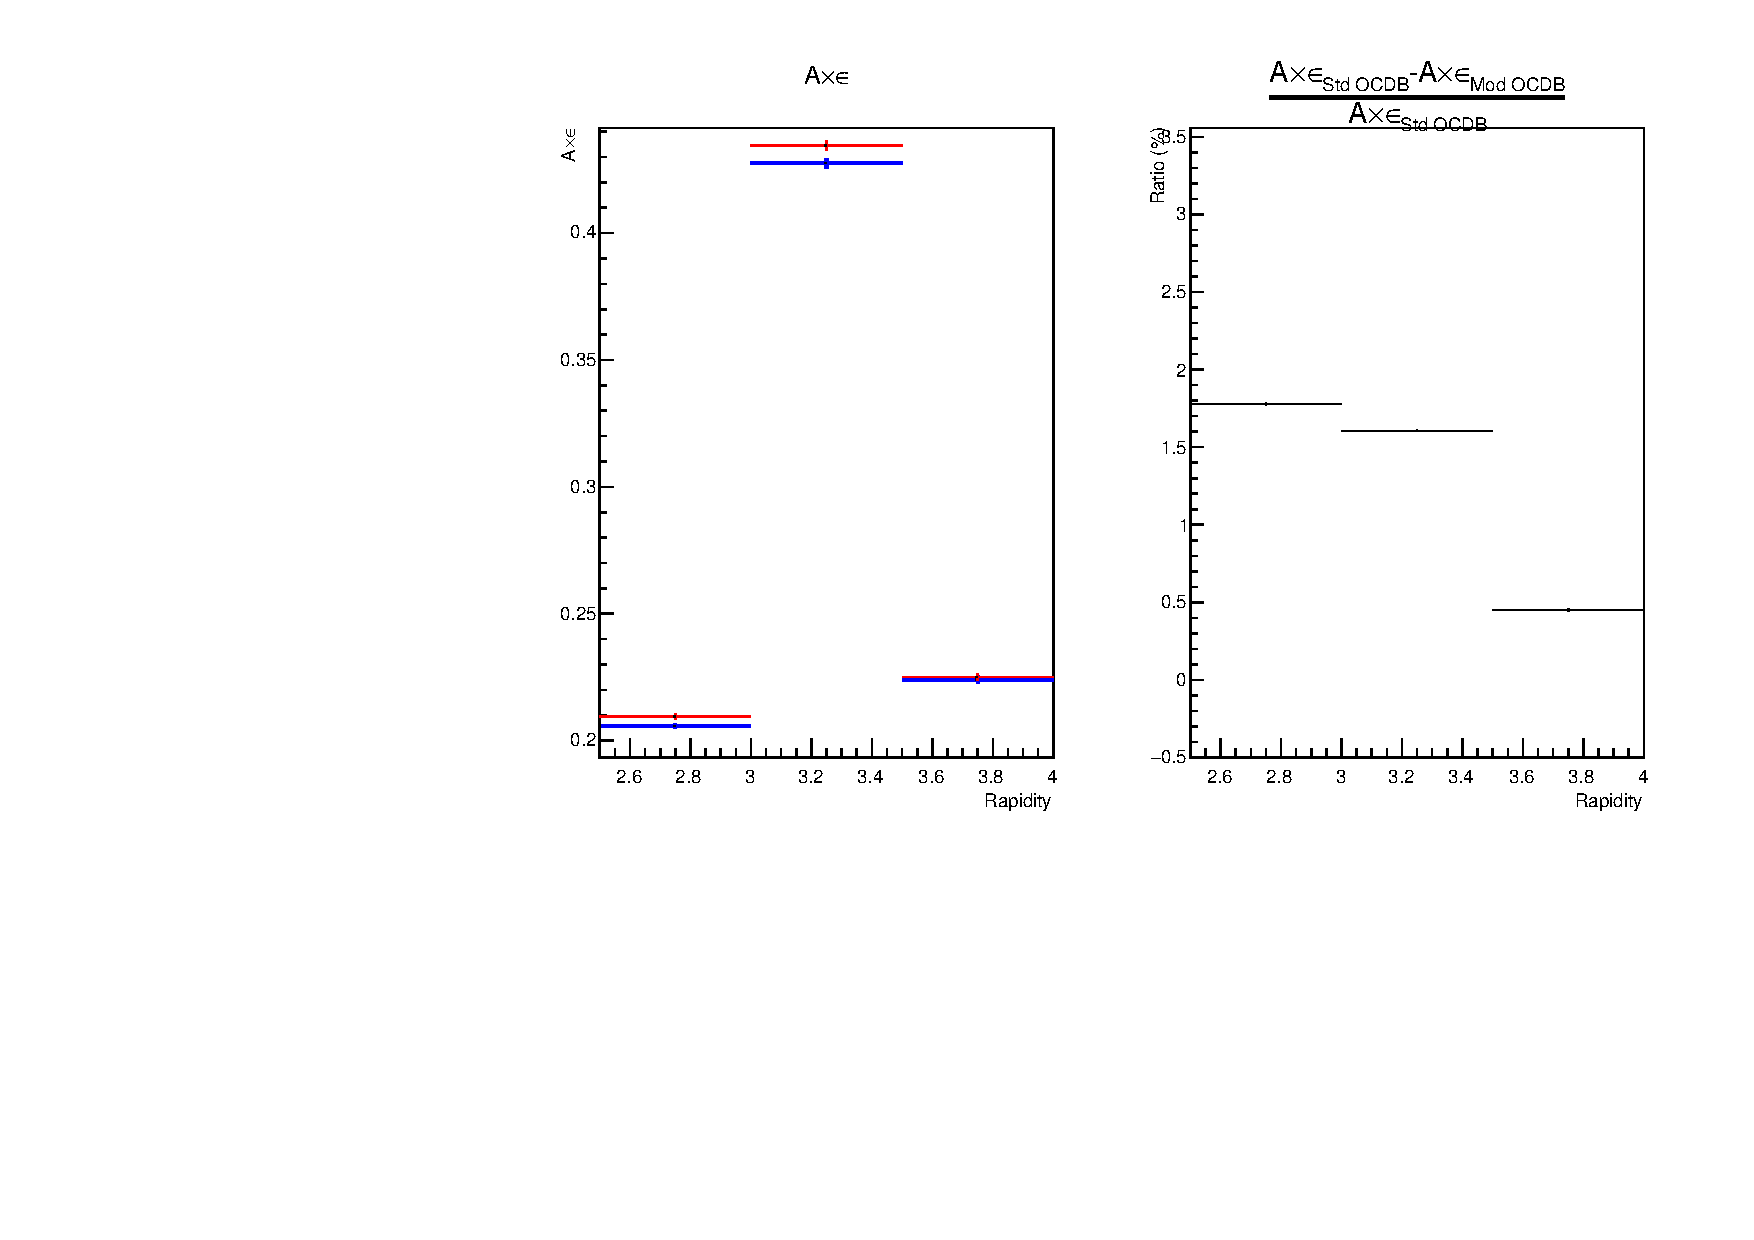
\includegraphics[width=13.cm]{/Trigger/AxEffSystError_NOCUT_correct.pdf}
\end{center} 
\caption{\label{fig:AxEffSyst} On the left hand side of the figure the $A\times\epsilon$ for real data (blue) and MC data (red) are reported for each rapidity bin. On the right hand side the relative difference, namely the systematic uncertainty, between the two integrals is reported.}
\end{figure}

\subsection{Trigger systematics summary}
The systematic uncertainties related to the muon trigger system are summarized in table \ref{tab:systSum}.

\begin{table}[!htb]
\centering
\begin{tabular}{ |c|c| }
 \hline
 $\eta$ interval&  $Syst_{RF}+Syst_{Eff}+Syst_{A\times\epsilon} (\%)$  \\
 \hhline{|=|=|}
 $2.5<\eta<3.0$&  $3.72\%$  \\
 \hline
 $3.0<\eta<3.5$&  $3.15\%$  \\
 \hline
 $3.5<\eta<4.0$&  $1.38\%$  \\
 \hline
\end{tabular}
\caption{Sum of the systematic uncertainties related to the muon trigger system.}
\label{tab:systSum}
\end{table}

\subsection{Centrality determination systematic}

\subsection{Other systematics}

\paragraph{}
As it has been presented in Section \ref{RAA}, other ingredients enter in the computation of the \ups nuclear modification factor.
The nuclear overlap function is determine through the ALICE centrality framework discussed in \cite{centframework}.
An uncorrelated systematic uncertainty of 3\% is set as a function of centrality while a correlated one of 3\% is set as a function of $y$.
The extrapolated $\sigma^{\rm pp}_{\ups}$ cross section is reported with a fully correlated systematic uncertainty of 9\% as a fonction of centrality and a fluctuation of 8-12\% is given as a function of $y$. 
Finally, a fully correlated systematic uncertainty of 1\% has been determined as a function of centrality and $y$.
The procedure is describe in the Section 4 of the \jpsi analysis note (\href{https://aliceinfo.cern.ch/Notes/node/486}{here}) referring to the same Pb-Pb data sample (LHC15o period).


\begin{table}[!htb]
\centering
\begin{tabular}{c|cc|cc}
\hline
sources & \multicolumn{2}{c|}{Centrality} & \multicolumn{2}{c}{$y$} \\
& value (\%) & type & value (\%) & type \\
\hline
Input MC     					& 1 			& I 		& 1-3 		& II \\
Signal extraction     				& 4-6 		& II 		& 4-7 		& II \\
Tracker						& 3 and 0-1 	& I and II 	& 1 and 3 		& I and II \\
Trigger						& 2  			& I 		& 2		 	& II \\
Matching 						& 1 			& I 		& 1 			& II \\
Centrality						& 0-5 		& II 		& 0			& I \\	
$F_{\rm{norm}}$          			& 1 			& I 		& 1 			& I \\
$\langle T_{\rm{AA}}\rangle$             & 3 			& II 		& 3 			& I \\
$\sigma^{\rm pp}_{\ups}$  		& 9 			& I 		& 8-12 		& II \\
\hline
\end{tabular}
\caption{\label{tablesys}Summary of the systematic uncertainties. Type I (II) refers to a correlated (uncorrelated) systematic.}
\end{table}